\documentclass[a4paper,12pt]{article}
\synctex=1
% math symbols
\usepackage{amssymb,amsmath}
% for different compilers
\usepackage{ifpdf}
% geometry of page
\usepackage[margin=2.3cm]{geometry}
\usepackage{fancyhdr}
% float pictures
\usepackage{wrapfig}

% if pdflatex, then
\ifpdf
 \usepackage[russian]{babel}
 \usepackage[utf8]{inputenc}
 \usepackage[unicode]{hyperref}
 \usepackage[pdftex]{graphicx}
% if xelatex, then
\else
% math fonts
 \usepackage{fouriernc}
% xelatex specific packages
 \usepackage[xetex]{hyperref}
 \usepackage{xltxtra}	% \XeLaTeX macro
 \usepackage{xunicode}	% some extra unicode support
 \defaultfontfeatures{Mapping=tex-text}
 \usepackage{polyglossia}	% instead of babel in xelatex
 \usepackage{indentfirst}	% 
 \setdefaultlanguage{russian}
% fonts
 \newfontfamily\cyrillicfont{SchoolBookC}
 \newfontfamily\cyrillicfontsf{TextBookC}
 \setmonofont{Consolas}
\fi

% several pictures in one figure
\usepackage{subfig}
% calc in TeX expressions
\usepackage{calc}
% nice pictures and plots
\usepackage{pgfplots,tikz,circuitikz}
% different libraries for pictures
\usetikzlibrary{%
  arrows,%
  calc,%
  patterns,%
  decorations.pathreplacing,%
  decorations.pathmorphing,%
  decorations.markings%
}
\tikzset{>=latex,%
  marrow/.style={postaction={draw,decorate,decoration={markings,
    mark=at position 0.6 with {\arrow{latex}}}}}}

\graphicspath{{./pics/}}

% colors of the hyperlinks
\hypersetup{colorlinks,%
  citecolor=blue,%
  urlcolor=blue,%
  linkcolor=red
}

\tolerance=1000
\emergencystretch=0.74cm

\numberwithin{equation}{section}


\newcommand{\nn}{\nonumber}
\newcommand{\pt}{\partial}
\newcommand{\eps}{\epsilon}
\newcommand{\vareps}{\varepsilon}
\newcommand{\const}{\mathrm{const}}
\newcommand{\com}[1]{{\Large{\texttt{{\color{red}(#1)}}}}}

\newcommand{\grad}{\mathrm{grad}\,}
\newcommand{\rot}{\mathrm{rot}\,}
\renewcommand{\div}{\mathrm{div}\,}
\newcommand{\vn}{\vec{\nabla}}

\pagestyle{fancy}
\rhead{\small\sffamily \emph{Электродинамика}}
\lhead{\small\sffamily \emph{Игорь Шендерович}}
\cfoot{-- \sffamily\thepage \ -- }
\rfoot{\tiny \sffamily версия от \today}
%\lfoot{\tiny \sffamily
%\href{mailto:shender.i@gmail.com}{shender.i@gmail.com}}
\lfoot{\tiny \textsf{Летний физический лагерь, июль--август 2011}}


\begin{document}

\thispagestyle{empty}
\begin{center}
  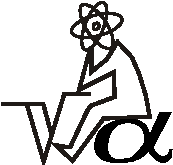
\includegraphics{logo}
  \vfill
  \LARGE{Электродинамика}\\[0.3cm]
  \Large{Игорь Шендерович}\\[0.3cm]
  {\large{\texttt{\href{mailto:shender.i@gmail.com}{shender.i@gmail.com}}}}\\[1cm]
  \large{Слушатели:\\[0.5cm]
    \hspace{2cm}\parbox[t]{0.4\textwidth}{
      Балашов Александр\\
      Борздун Наталья\\
      Грачёв Дмитрий\\
      Жаровов Дмитрий\\
      Косицын Александр\\
      Максимишин Дмитрий\\
      Маслов Артём\\
      Матюшин Георгий\\
      Михайлов Кирилл
      }\hspace{1cm}\parbox[t]{0.4\textwidth}{
       Никитин Денис\\
       Свирина Анна\\
       Смирнов Иван\\
       Терехов Антон\\
       Толстопятов Всеволод\\
       Трофимов Павел\\
       Чурилова Мария\\
       Шалымов Роман
      }
    }
  \vfill
  
  \normalsize{\textsf{XVII Летняя Физическая Школа\\
  2011}}
\end{center}

\clearpage


\section{Введение.}
\label{sec:intro}

Мы собираемся изучать электродинамику --- науку о движении зарядов,
токов и электромагнитных полей. Прежде чем углубляться в теорию,
поймём, какие именно экспериментальные, наблюдаемые явления мы хотим
объяснить. 

\subsection{Экспериментальные факты.}
\label{sec:exp_facts}

Чтобы понимать, к чему мы стремимся, опишем ряд экспериментальных
явлений, которые мы хотим объяснить. 

\begin{enumerate}
\item Отклонение стрелки компаса при прохождении по лежащему рядом
  проводнику электрического тока. Это явление было замечено в 1820
  году датским физиком Эрстедом. Стрелка компаса отклоняется тем
  сильнее, чем больший ток проходит по проводу.
\item Притяжение двух электрических проводов, по которым идёт в одну
  сторону электрический ток. Отталкивание этих проводов, если токи
  текут в противоположные стороны.
\item Существование электромагнитных волн --- то есть, например,
  света. Как распространяется свет? С какой скоростью? Можно ли
  предсказать, какова будет скорость света в данной среде?
\item Возникновение переменной ЭДС в замкнутом проводнике, когда сквозь него
  пролетает магнит.
\end{enumerate}

\subsection{Стратегия.}
\label{sec:strategy}

Как мы будем действовать? Сходу кажется, что в нашем распоряжении нет
никаких инструментов для объяснения этих фактов. Действительно, что мы
знаем об электричестве в целом? Мы знаем, что есть электростатика, то
есть, наука о взаимодействии \textit{статических} зарядов. В рамках
этой науки мы можем установить такие законы, как закон Кулона (о силе
притяжения между двумя точечными зарядами), закон Гаусса (о потоке
электрического поля в зависимости от электрического заряда) и ряд
других. Могут ли они нам помочь в задаче описания движущихся зарядов и
движущихся полей? 

Ключевой особенностью здесь является концепция \textbf{поля}. На
примере электростатики мы видим, что поле появляется уже в простейшей
задаче о взаимодействии двух точечных зарядов. Действительно,
известно, что точечный заряд $q$ создаёт вокруг себя поле,
напряжённость которого выражается формулой 

\begin{equation}
  \label{eq:q_E}
  \vec{E} (\vec{r}) = k \frac{q \vec{r}}{r^3}.
\end{equation}

Видно, что вектор $\vec{E}$ существует в любой точке пространства, вне
зависимости от того, насколько далеко мы отошли от заряда. Это
позволяет ввести понятие \textit{векторного поля} --- вида материи,
который существует при наличии источника. В данном случае источником
электрического поля является заряд $q$. Позднее мы увидим, что
магнитное поле, несмотря на отсутсвие одиночных источников, также
допускает такую интерпретацию. С этого момента мы будем говорить не о
напряжённости $\vec{E}$, а об электрическом (или магнитном) поле
$\vec{E}(x,y,z,t)$ (или $\vec{B}(x,y,z,t)$). Заметим, что в нашем
описании поле может зависеть как от точки пространства, так и от
времени.

Поскольку вектор определяется своими проекциями, то задать векторное
поле --- то же самое, что задать три его проекции. Таким образом,
электрическое поле $\vec{E}$ --- три функции четырёх переменных. 

Таким образом, для того, чтобы научиться описывать электромагнитные
явления, нужно будет научиться работать с полями. Этому будет посвящён
раздел \ref{sec:vector_analysis}. Далее, в разделе
\ref{sec:electrostatics} мы вспомним электростатику и перепишем её
основные формулы на языке векторного анализа. После этого в разделе
\ref{sec:maxwell} мы попробуем перейти к движущимся зарядам путём
перехода в движущуюся инерциальную систему отсчёта.

В разделе \ref{sec:magnetostatics} мы посмотрим на получившуюся в
итоге \textbf{магнитостатику} --- науку о магнитных полях в
статическом приближении. Далее, мы встроим в нашу картину мира
электромагнитные волны (в разделе \ref{sec:em_waves}) и построим
полную систему уравнений Максвелла. 

\section{Векторный анализ.}
\label{sec:vector_analysis}

Итак, приступим к описанию концепции поля. Разумеется, в природе
существуют различные поля, не только электромагнитные. 

Рассмотрим, например, поле температур $T(x,y,z,t)$. Это
тоже поле (т.к. температуру можно определить в любой точке
пространства), но \textit{скалярное}, поскольку температура не имеет
направления, а определяется лишь числовым значением. 

Другой пример векторного поля, более приближенный к реальности ---
поле скоростей жидкости. Каждой <<частице>> движущейся жидкости можно
сопоставить векторную функцию $\vec{v}(\vec{r},t)$, которая описывает
скорость данной частички. По определению, это векторное поле
скоростей. Мы увидим в дальнейшем, что многие свойства этого поля
жидкости переносятся и на электродинамику. 

Электрические и магнитные (или просто электромагнитные) поля устроены
довольно сложно, но при этом связь между значениями полей в двух
соседних точках довольно проста. Задача наших упражнений --- вывести
эту связь в наиболее общем виде. 

\begin{wrapfigure}{r}{40mm}
  \vspace{-1cm}
  \begin{center}
    \begin{tikzpicture}
      \draw[thick,marrow] (0,3) to [out=10,in=200] (3,3.2);
      \draw[thick,marrow] (0,2.5) to [out=0,in=195] (3,2.6);
      \draw[thick,marrow] (0,2) to [out=0,in=190] (3,2.1);
      \draw[thick,marrow] (0,1.5) to [out=0,in=185] (3,1.6);
    \end{tikzpicture}
  \end{center}
  \vspace{-1cm}
  \label{fig:force_lines}
\end{wrapfigure}

Как можно зрительно представлять поля? Лучше всего это делать с
помощью \textbf{силовых линий} --- таких линий, касательные к которым в
каждой точке будут давать направление вектора напряжённости в этой
точке. 

Чтобы изобразить на подобной картинке величину модуля вектора
напряжённости, можно условиться рисовать линии гуще в тех местах, где
абсолютная величина этого вектора больше. 

\subsection{Поток.}
\label{sec:flux}

Векторные поля обладают двумя очень важными характеристиками, которые
мы будем использовать при описании. Первая из них --- \textbf{поток}. 

Рассмотрим, к примеру, поток жидкости через некоторую ограниченную
поверхность. Можно задать себе вопрос --- сколько жидкости втекает
(вытекает) через эту поверхность площади $S$? 

\begin{wrapfigure}{r}{40mm}
  \begin{center}
    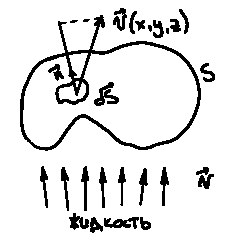
\includegraphics[width=4cm,height=4cm]{flux.pdf}
  \end{center}
  \label{fig:flux}
\end{wrapfigure}

Это количество можно посчитать следующим образом. Разобъём нашу
поверхность на много кусочков с площадью $dS$ каждый. К каждому
кусочку проведём вектор нормали $\vec{n}$ (так, чтобы он смотрел
наружу поверхности, а не внутрь). Тем самым, у каждого кусочка площади
будет задана ориентация. Для краткости совокупность данных о площади
кусочка и векторе нормали можно записывать в виде одного вектора
$d\vec{S}$ --- это вектор, по модулю равный $dS$, с направлением,
совпадающим с $\vec{n}$.

Спроецируем на направление этого вектора наше поле $\vec{v}$. Операция
проектирования проще всего выглядит как скалярное произведение
$\vec{v} \cdot d \vec{S}$. Действительно, по определению, скалярное
произведение равно $d\Phi = v \cdot dS \cdot \cos \alpha$, где $\alpha$ ---
угол между вектором $\vec{v}$ и нормалью $\vec{n}$. Теперь
просуммируем подобные выражения по всей поверхности, иными словами,
проинтегрируем по ней:

\begin{equation}
  \label{eq:def_flux}
  \Phi \equiv \int_S \vec{v} \cdot d \vec{S}.
\end{equation}

По определению, это скалярное произведение и называется потоком $\Phi$ 
векторного поля $\vec{v}$. Можно интерпретировать это определение и
таким способом: поток векторного поля равен среднему значению
нормальной компоненты поля $\vec{v}$, умноженному на величину площади
$S$. 

Если, например, поле устроено так, что не зависит от конкретной точки
(всюду постоянное поле), то формула для расчёта потока может быть
сильно упрощена. Пусть, скажем, поле всюду направлено по нормали к
поверхности (пример --- электрическое поле точечного заряда, а
поверхность --- сфера). Тогда в любой точке скалярное произведение
превращается в обычное (т.к. $\cos 0 = 1$), и функцию $v$ можно
вынести за знак интеграла. Интеграл же от $dS$ даст просто площадь
поверхности. Таким образом, в этом простейшем случае поток станет
равен $\Phi = vS$. 

В более сложных случаях (которые обычно и встречаются в природе),
вычисление потока по определению --- довольно сложная задача. К
счастью, у нас будет \textbf{теорема Гаусса}, которая позволяет свести
вычисление потока к относительно простым операциям. 

\subsection{Циркуляция.}
\label{sec:curl}

Опять представим себе поле скоростей, описывающее поток
жидкости. Зададимся таким вопросом: циркулирует ли эта жидкость? Иными
словами, существует ли её вращательное движение вдоль некоторого
замкнутого геометрического контура? 

\begin{wrapfigure}{r}{40mm}
  \vspace{-1.5cm}
  \begin{center}
    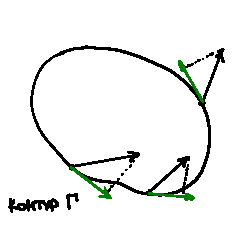
\includegraphics[width=4cm,height=4cm]{curl.pdf}
  \end{center}
  \vspace{-0.7cm}
  \label{fig:curl}
\end{wrapfigure}


По определению, \textbf{циркуляцией} $C$ называется скорость жидкости вдоль
контура, умноженная на длину этого контура. Как и в случае с потоком,
можно думать про эти величины как про средние; более аккуратное
определение можно получить, опять пользуясь понятием проекции. 

Рассмотрим участок контура длиной $dl$. С ним, как и с кусочком
площадки, можно связать направление. Рассмотрим вектор $d\vec{l}$ ---
это вектор, модуль которого равен $dl$, а направление совпадает с
направлением касательной в данной точке. Теперь спроецируем наше
векторное поле $\vec{v}$ на этот вектор $d\vec{l}$. Сделать это можно
так же, как и в случае с потоком, т.е. взять скалярное
произведение. Теперь просуммируем это по всему контуру:

\begin{equation}
  \label{eq:curl}
  C \equiv \oint_\Gamma \vec{v} \cdot d \vec{l}.
\end{equation}

Пользуясь понятиями потока и циркуляции, мы опишем все законы
электродинамики, т.е. получим уравнения Максвелла. 

\subsection{Произведение векторов.}
\label{sec:vector_product}

Разберём подробнее операции с векторами. Нам понадобится умение
перемножать вектора двумя способами, дифференцировать их и
интегрировать. 

Два вектора $\vec{a}$ и $\vec{b}$ можно перемножить двумя способами:
скалярно и векторно. \textbf{Скалярное произведение} определяется через
компоненты этих векторов:

\begin{equation}
  \label{eq:def_scalar_product}
  \vec{a} \cdot \vec{b} \equiv a_x b_x + a_y b_y + a_z b_z.
\end{equation}

С помощью скалярного произведения можно также определить модуль
вектора: это корень из скалярного произведения вектора на самого себя.

\begin{equation}
  \label{eq:def_modulus_vector}
  |a| \equiv \sqrt{\vec{a} \cdot \vec{a}}.
\end{equation}

Также можно образовать \textbf{векторное произведение}: такое
произведение двух векторов, результатом которого является снова
вектор. Модуль этого вектора равен

\begin{equation}
  \label{eq:def_cross_product}
  | \vec{a} \times \vec{b}| = |\vec{a}| |\vec{b}| \sin \alpha,  
\end{equation}
а направление задаётся правилом правой руки. Угол $\alpha$ --- угол
между векторами. 

\begin{wrapfigure}{r}{40mm}
  \vspace{-0.7cm}
  \begin{center}
    \begin{tikzpicture}
      \draw[very thick,red,->] (0,0) -- (1,1) node[right] {$\vec{a}$};
      \draw[very thick,blue,->] (0,0) -- (2.5,-1) node[right]
      {$\vec{b}$};
      \draw[very thick,green!70!black,->] (0,0) -- (0,2.5) node[right]
      {$\vec{a} \times \vec{b}$};
      \draw[very thick,green!70!black,->] (0,0) -- (0,1) node[right]
      {$\vec{n}$};
      \draw[thick] (0.4,-0.15) arc (-30:45:0.4cm);
      \draw (0.65,0.1) node {$\alpha$};
    \end{tikzpicture}
  \end{center}
  \label{fig:curl}
  \vspace{-1cm}
\end{wrapfigure}

Свойства этого произведения довольно просты. Во-первых, если вектора
$\vec{a}$ и $\vec{b}$ коллинеарны, то $\vec{a} \times
\vec{b}=0$. Во-вторых, модуль этого вектора совпадает с площадью
параллелограмма, натянутого на вектора $\vec{a}$ и $\vec{b}$.

А можно ли записать определение векторного произведения в координатах,
подобно \eqref{eq:def_scalar_product}? Оказывается, можно. Именно, 

\begin{eqnarray}
  \label{eq:def_cross_product_components}
  \nn
  (\vec{a} \times \vec{b})_x &=& a_y b_z -a_z b_y,\\
  (\vec{a} \times \vec{b})_y &=& a_z b_x -a_x b_z,\\
  \nn
  (\vec{a} \times \vec{b})_z &=& a_x b_y -a_y b_x.
\end{eqnarray}

Запомнить это правило довольно просто: для i-ой компоненты нужно
устроить циклическую перестановку из индексов (xyz), где нужный индекс
стоит на i-ом месте. 

Понять, откуда взялось это правило, довольно просто. Рассмотрим три
орта $\vec{i},\vec{j},\vec{k}$. Применяя к ним правило
\eqref{eq:def_cross_product}, получим, что $\vec{i} \times \vec{j} =
\vec{k}$, \ldots. Расписывая вектор $\vec{a} = a_x \vec{i} + a_y
\vec{j} + a_z \vec{k}$, а вектор $\vec{b}$ аналогично, получим
требуемые свойства \eqref{eq:def_cross_product_components}. 

\subsection{Градиент. Оператор $\nabla$.}
\label{sec:gradient}

Предположим, что у нас имеется для начала скалярное поле, типа поля
температур. Мы хотим как-то описать изменение температуры $T(x,y,z,t)$
в пространстве. В отличие от похожей задачи --- изменения температуры
по времени --- нам нужно дифференцировать не по времени, а придумать
что-то другое, более подходящее к данному случаю.

Понятно, что если бы у нас была одна координата, то сработала бы
производная $dT/dx$, потому что именно она бы определяла скорость
изменения температуры вдоль оси $x$. В данном случае нам понадобятся
три производных 

\begin{equation}
  \label{eq:def_grad_1}
  \frac{\pt T}{\pt x}, \quad   \frac{\pt T}{\pt y}, \quad   \frac{\pt
    T}{\pt z},
\end{equation}
из которых можно сделать вектор. Вектор можно соорудить естественным
способом. Вспомним, что у нас есть три орта
$\vec{i},\vec{j},\vec{k}$. Построим вектор \textbf{градиента} по такому
правилу:

\begin{equation}
  \label{eq:def_grad_2}
  \grad T (x,y,z) \equiv \nabla T \equiv \frac{\pt T}{\pt x} \vec{i} +  \frac{\pt T}{\pt y}
  \vec{j} +  \frac{\pt T}{\pt z} \vec{k}.
\end{equation}

Таким образом, можно сказать, что градиент скалярного поля --- это
аналог производной, только в числе измерений больше одного. 

Заметим, что градиент, будучи вектором, явно зависит от
направления. Это сооветствует тому факту, что температура в разных
направлениях пространства может вестии себя по-разному. Таким образом,
градиент температуры $\grad T$ --- векторное поле, образованное из скалярного
поля самой температуры $T$.

Физический смысл градиента такой: в каждой точке пространства он
указывает направление, в котором температура меняется быстрее всего. 

Оказывается, что у градиента есть ещё одна интерпретация. Она ведёт к
обобщению известной теоремы \textbf{Ньютона--Лейбница}. Эта теорема
устроена примерно так. Представим себе, что у нас есть материальная
точка, двигающаяся в пространстве. Её координаты мы будем
характеризовать радиус--вектором $\vec{r}(t)$. Вычислим скорость этой
материальной точки; по определению, она равна $\vec{v} (t) = d
\vec{r}(t) / dt$. Что получится, если мы теперь проинтегрируем эту
скорость по времени от момента $t_1$ до $t_2$? 

\begin{equation}
  \label{eq:newton_leibnitz}
  \int_{t_1}^{t_2} \vec{v}(t) \, dt = \int_{t_1}^{t_2}
  \frac{d\vec{r}(t)} {dt} \, dt = \int_{t_1}^{t_2} d\vec{r}(t) =
  \vec{r}(t_2) - \vec{r}(t_1) = \Delta \vec{r}.
\end{equation}

\begin{wrapfigure}{r}{40mm}
  \vspace{-1.2cm}
  \begin{center}
    \begin{tikzpicture}
      \draw[thick,decorate,decoration=ticks] (0,0) to[out=80,in=250]
      (3,3);
      \draw[thick] (0,0) node[below] {1} to[out=80,in=250] (3,3)
      node[right] {2};
      \draw[blue,->] (2.5,0.5) node[below] {$\Delta\vec{l}$}
      to[out=150,in=300] (0.95,1.2);
      \draw[thick,blue,->] (0.77,1.15) -- ++(0.3,0.8) node[above] {$\vec{f}$};
    \end{tikzpicture}
  \end{center}
  \label{fig:curve_int}
\end{wrapfigure}


То есть, если проинтегрировать скорость, получится перемещение. Более
общо: если проинтегрировать производную некоторой функции $f(t)$,
получится изменение этой самой функции $f(t)$. 

Эта теорема естественным образом ограничена на прямую линию (интеграл
вдоль прямой). Что будет, если мы захотим проинтегрировать что-нибудь
(а точнее, какой--нибудь вектор) вдоль произвольной кривой? 

В этом случае нам нужно описать процедуру интегрирования вдоль
кривой. Рассмотрим кусочек дуги кривой $\Delta l_i$. Пускай значение функции
на нашем кусочке равно $f_i$. Тогда интегралом вдоль кривой $C$
называется такое выражение:

\begin{equation}
  \label{eq:def_curve_int_1}
  \int_C  \vec{f} \cdot d\vec{l} \equiv \lim_{N\to \infty} \sum_{i=0}^N f_i \Delta l_i. 
\end{equation}

В общем, это что-то, аналогичное стандартному определению интеграла,
только нужно учитывать, что $f_i$ --- значение функции на этом
отрезке. В нашем случае вместо скаляра $f_i$ уместно взять скалярное
произведение 

\begin{equation}
  \label{eq:def_curve_int_2}
  \grad \phi \cdot d\vec{l}_i.
\end{equation}

Мы уже знаем, что градиент показывает, насколько быстро меняется
функция в данном направлении. Таким образом, если мы спроецируем
градиент на какое-то выделенное направление, мы получим скорость
изменения функции в этом направлении. Проецирование делатся в точности
скалярным произведением \eqref{eq:def_curve_int_2}. Таким образом,
уравнение \eqref{eq:def_curve_int_2} даёт изменение скалярного поля в
направлении $d\vec{l}_i$: $\phi(i+1) - \phi(i)$, где $\phi(i)$ ---
значение поля в точке $i$. Суммируя все такие изменения, получаем, что
сумма \eqref{eq:def_curve_int_1} превращается в конечное изменение 

\begin{equation}
  \label{eq:def_curve_int_3}
  \int_C \grad \phi \cdot d\vec{l} = \phi(2) - \phi(1).
\end{equation}

Таким образом, мы видим, что у градиента есть такой смысл: будучи
проинтегрирован по какой-либо кривой, он даёт изменение конечное
изменение скалярной функции вдоль этой кривой. 

Заметим попутно, что интеграл от градиента, очевидно, не зависит от
кривой, вдоль которой мы интегрируем. Действительно, правая часть
уравнения \eqref{eq:def_curve_int_3} зависит только от значений поля
$\phi$ в точках 1 и 2, и больше не от чего. Очевидно, что значения
поля в этих точках не зависят от того, по какому пути мы в эти точки
пришли. 

Что будет, если мы придём из точки 1 в точку 2 по красному пути, а
уйдём обратно по синему? Мы опишем замкнутый контур. 

\begin{wrapfigure}{r}{40mm}
  \vspace{-0.75cm}
  \begin{center}
    % 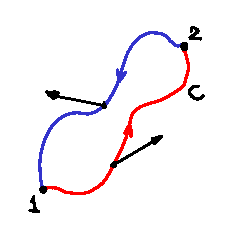
\includegraphics[width=4cm,height=4cm]{path_indep.pdf}
    \begin{tikzpicture}
      \draw[thick,red,marrow] (0,0) to[out=-10,in=270] (1,1)
      to[out=90,in=270] (3,3);
      \draw[thick,->] (1,1) -- ++ (1,-0.2);
      \draw[thick,blue,marrow] (3,3) to[out=140,in=120] (0,0);
      \draw[fill=black] (0,0) circle (0.05cm);
      \draw[fill=black] (3,3) circle (0.05cm);
    \end{tikzpicture}
  \end{center}
  \vspace{-0.7cm}
  \label{fig:path_indep}
\end{wrapfigure}

Пройдём по красному контуру от точки 1 до точки 2. При этом значение
интеграла \eqref{eq:def_curve_int_3} даст нам, как и положено, $\phi(2)
- \phi(1)$. Теперь пройдём от точки 2 до точки 1 по синему
контуру. Интеграл даст на этот раз $\phi(1) - \phi(2)$. В итоге наших
прогулок по разноцветным контурам мы придём обратно в точку 1, при
этом значение интеграла по замкнутому контуру будет равно 0. Опять же,
заметим, что он конкретной формы этого контура ничего не зависит. 

Таким образом, мы доказали, что интеграл от градиента по замкнутому
контуру равен нулю, и от контура не зависит. Или, вспоминая
определение циркуляции \eqref{eq:curl}, мы доказали, что циркуляция
градиента равна нулю.

\begin{equation}
  \label{eq:int_grad}
  \oint \grad \phi \cdot  d\vec{l} =0.
\end{equation}

В дальнейшем этот факт нам поможет. 

Напоследок продемонстрируем один трюк, ради которого (отчасти) это всё
и затевалось. Обозначим \emph{формально} буквой $\nabla$ такую
операцию:

\begin{equation}
  \label{eq:def_nabla}
  \vec{\nabla} \equiv \frac{\pt}{\pt x} \vec{i} +  \frac{\pt}{\pt y}
  \vec{j} +  \frac{\pt}{\pt z} \vec{k}.
\end{equation}

Буква $\vec{\nabla}$ теперь играет роль \textbf{оператора градиента},
т.е. не самостоятельной буквы, а чего-то, что имеет смысл только в
паре с функцией, к которой она применяется. Оператор градиента
<<ждёт>> функцию, которую ему надо продифференцировать. Из формулы
\eqref{eq:def_grad_2} видно, что градиент можно получить, действуя
оператором градиента на наше скалярное поле.

Очевидно, что, будучи вектором, оператор $\vec{\nabla}$ может быть применён
не только к скалярам (типа поля температуры), но и к векторам,
порождая объекты с очень прозрачным физическим смыслом. 

\subsection{Дивергенция.}
\label{sec:divergence}

Первое, что мы можем сделать с вектором $\vec{\nabla}$ и каким-то
векторным полем $\vec{A}$ --- скалярно их перемножить. Как следует из
определения, должен получиться скаляр. Посмотрим, так ли это.

\begin{equation}
  \label{eq:def_divergence}
  \div \vec{A} \equiv \vec{\nabla} \cdot \vec{A} = \frac{\pt}{\pt x}
  A_x +  \frac{\pt}{\pt y} A_y +  \frac{\pt}{\pt z} A_z = \frac{\pt
    A_x}{\pt x} +  \frac{\pt A_y}{\pt y} +  \frac{\pt A_z}{\pt z}.
\end{equation}

Скалярная величина, которую мы получили, называется
\textbf{дивергенцией}. Фактически, оператор $\vec{\nabla}$, скалярно
умноженный на $\vec{A}$, дифференцирует каждую из компонент вектора
$\vec{A}$ по соответствующей координате и складывает результаты без
учёта направления. Этим он и отличается от градиента: градиент,
напомним, даёт вектор. 

Итак, если градиент скалярному полю сопоставляет векторное, то
дивергенция векторному полю сопоставляет скалярное. 

Нет ли случайно у дивергенции какого-нибудь внятного физического
смысла? Разумеется, есть, иначе зачем бы она нам понадобилась!

Чтобы понять этот физический смысл, нам понадобится вспомнить понятие
потока \eqref{eq:def_flux}. Рассмотрим какое--нибудь тело, через
которое проходит векторное поле. Разобъём тело на маленькие одинаковые
кубики. Рассмотрим маленький кубик со сторонами $\Delta x$, $\Delta
y$, $\Delta z$. Пускай в пространстве есть какое-то векторное поле
$\vec{A}$. Вычислим его поток (наружу) через поверхность этого кубика.

\begin{wrapfigure}{r}{40mm}
  \begin{center}
    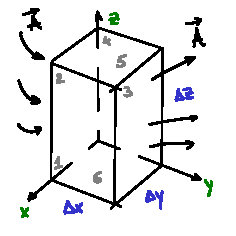
\includegraphics[width=4cm,height=4cm]{div.pdf}
  \end{center}
  \label{fig:div}
\end{wrapfigure}

У поверхности кубика 6 граней. Можно вычислить поток через каждую из
них. Поскольку грани --- маленькие квадраты, вычисление будет
несложным. Например, поток через грань 1 равен

\begin{equation}
  \label{eq:theorem_divergence_1}
  \Phi_1 = -\int A_y (x,y,z) dx dz.
\end{equation}

(знак минус появился от того, что в грань 1 наше поле \emph{входит},
так что поток \emph{наружу} будет со знаком минус). Это выражение
можно упростить: так как мы считаем наш кубик маленьким, то можно
считать, что на грани функция $A_y$ примерно постоянная; раз так, то
её можно вытащить за знак интеграла. Останется лишь интеграл по
площади грани, который равен собственно площади $\Delta x \Delta z$. 

Итого, получаем, что поток через грань 1 равен

\begin{equation}
  \Phi_1 = - A_y \Delta x \Delta z. 
\end{equation}

Рассмотрим теперь поток наружу через грань 3:

\begin{equation}
  \Phi_3 = \int A_y (x,y + \Delta y,z) dx dz = A_y (x,y+\Delta y,z)
  \Delta x \Delta z.
\end{equation}

Сложим теперь потоки $\Phi_1 + \Phi_3$ --- это логично сделать, потому
что у них есть много общего. 

\begin{equation}
  \label{eq:theorem_divergence_2}
  \Phi_1 + \Phi_3 = \Delta x \Delta z \left(A_y(y+\Delta y) - A_y
    (y)\right) \approx \Delta x \Delta z \Delta y \frac{\pt A_y}{\pt y}.
\end{equation}

Здесь мы заменили разность полей на двух гранях производной потому,
что кубик считается маленьким и такая замена не внесёт существенной
ошибки. Аналогичные операции можно провернуть и для остальных четырёх
граней; ответ для полного потока $\Phi$ совсем не удивителен:

\begin{equation}
  \label{eq:theorem_divergence_3}
  \Phi = \Delta x \Delta y \Delta z
  \left(
    \frac{\pt A_x}{\pt x} + 
    \frac{\pt A_y}{\pt y} + 
    \frac{\pt A_z}{\pt z}
  \right) = \Delta V \div \vec{A}. 
\end{equation}

Таким образом, физический смысл дивергенции такой: это поток
векторного поля, отнесённый к единице объёма $\Delta V$. Можно
сказать, что дивергенция меряет <<удельную величину>> потока, измеряя,
насколько мощный источник поля мы имеем. 

Более того, если мы теперь проинтегрируем равенство
\eqref{eq:theorem_divergence_3} по всему объёму тела и вспомним
определение потока \eqref{eq:def_flux}, мы получим ещё
одно соотношение, известное как \textbf{теорема Гаусса--Остроградского}:

\begin{equation}
  \label{eq:theorem_gauss_ostograd}
  \int_V \div \vec{A}\, dV =  \int_S \vec{A} \cdot  d\vec{S}.
\end{equation}

Заметим, что это соотношение чем-то похоже на теорему о градиенте
\eqref{eq:def_curve_int_3}: в правой части стоит что-то, размерности
на единицу меньшей, чем в левой части. Теперь если вы хотите сосчитать
поток какого--нибудь поля, у вас есть два варианта: либо вы честно его
считаете и берёте поверхностный интеграл, либо вы считаете дивергенцию
и берёте интеграл по объёму. Точно то же самое было в случае
градиента: либо считать интеграл вдоль кривой, либо считать приращение
функции вдоль этой же кривой.

Вскоре мы выясним, что есть ещё одна теорема похожего типа. Но для
начала посмотрим, на что ещё может сгодиться оператор $\vn$. 

\subsection{Ротор.}
\label{sec:curl}

Что ещё можно смастерить из оператора $\vec{\nabla}$ и вектора?
Помимо скалярного произведения, которое приводит к дивергенции, можно
сделать векторное произведение; в итоге получится вектор. Какие же у
него будут компоненты? Из формул \eqref{eq:def_cross_product} и
\eqref{eq:def_nabla} получаем: 

\begin{eqnarray}
  \label{eq:def_curl}
  \nn
  (\vec{\nabla} \times \vec{A})_x &=& \frac{\pt A_z}{\pt y} -  \frac{\pt
    A_y}{\pt z},\\
  (\vec{\nabla} \times \vec{A})_y &=& \frac{\pt A_x}{\pt z} -  \frac{\pt
    A_z}{\pt x},\\
  \nn
  (\vec{\nabla} \times \vec{A})_z &=& \frac{\pt A_y}{\pt x} -  \frac{\pt
    A_x}{\pt y}.
\end{eqnarray}

Вектор $\rot \vec{A} \equiv \vn \times \vec{A}$ называют
\textbf{ротором} или \textbf{вихрем}. Название выбрано неслучайно:
физический смысл этого вектора тесно связан с вихрями в потоке
жидкости (или в любом другом векторном поле).

Можно ли как-то выяснить физический смысл ротора аналогично
дивергенции и градиенту? Сейчас мы получим нечто, аналогичное теореме
Гаусса--Остроградского. Если в случае с дивергенцией мы интегрировали
поле по поверхности маленького кубика, то в случае с ротором надо
интегрировать по границе маленького квадрата (так подсказывает наша
интуиция).

\begin{wrapfigure}{r}{40mm}
  \begin{center}
    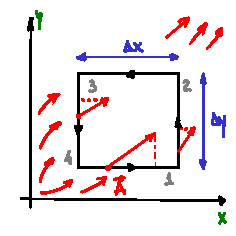
\includegraphics[width=4cm,height=4cm]{stokes.pdf}
  \end{center}
  \label{fig:stokes}
\end{wrapfigure}

Рассмотрим, например, квадрат, расположенный в плоскость $xy$ со
сторонами $\Delta x$, $\Delta y$. Вычислим циркуляцию поля $\vec{A}$
по этому квадрату. Также как и в случае с потоком, полная циркуляция
складывается из циркуляций по каждому ребру. Посмотрим, например, на
ребро 1. Циркуляция по нему равна

\begin{equation}
  \label{eq:theorem_curl_1}
  C_1 = \int A_x (x,y) d x = A_x (x,y) \Delta x. 
\end{equation}

Здесь мы, как и в предыдущем пункте, воспользовались тем, что
квадратик маленький, а значит, поле на его ребре можно считать
постоянным вдоль ребра. Коль так, то поле можно вынести за знак
интеграла, ну а интеграл от $dx$ даст просто длину ребра. Проводя
аналогичную операцию для остальных рёбер, получим в сумме для
циркуляции

\begin{equation}
  \label{eq:theorem_curl_2}
  C_{xy} = C_1 + \ldots C_4 = \Delta x
  \left(
    A_x (x,y) - A_x(x,y+\Delta y)
  \right) + \Delta y
  \left(
    A_y (x+\Delta x, y) - A_y (x,y)
  \right).
\end{equation}

Раскладывая разность в скобках (наш контур считается малым), получим:

\begin{equation}
  \label{eq:theorem_curl_3}
  C_{xy} = \Delta x \Delta y \left(\frac{\pt A_y}{\pt x} - \frac{\pt A_x}{\pt y}\right).
\end{equation}

У нас получилось, что циркуляция поля вдоль контура, лежащего в
плоскости $xy$ равна площади этого контура $\Delta x \Delta y$,
умноженной на компоненту $z$ ротора поля $C$ (см. формулу
\eqref{eq:def_curl}). Компонента $z$ в данном случае --- нормальная
составляющая ротора по отношению к плоскости $xy$. Таким образом,
можно написать, что
\begin{equation}
  \label{eq:theorem_curl_4}
  \oint \vec{A} \cdot d\vec{l} = \rot \vec{A} \cdot \vec{n}\, \Delta S.
\end{equation}

Если теперь просуммировать циркуляции по всем маленьким контурам на
нашей поверхности $S$, получится \textbf{теорема Стокса}:

\begin{equation}
  \label{eq:theorem_curl_5_stokes}
  \oint \vec{A} \cdot d \vec{l} = \int_S \rot \vec{A} \cdot \vec{n} \,
  dS = \int_S \rot \vec{A} \cdot d\vec{S}.
\end{equation}

Опять, по аналогии с дивергенцией, заметим, что теорема связывает
нечто одномерное по сути (циркуляцию) с чем-то двумерным (интеграл по
поверхности от ротора). В каком-то смысле, теорема о градиенте
\eqref{eq:def_curve_int_3}, теорема Гаусса--Остроградского
\eqref{eq:theorem_gauss_ostograd} и теорема Стокса
\eqref{eq:theorem_curl_5_stokes} --- частные случаи одного более
общего соотношения, про которое здесь мы говорить не будем. 

\subsection{Манипуляции с $\nabla$.}
\label{sec:nabla}

Сейчас мы начнём получать дивиденды от записи векторных операций через
оператор $\vn$. Попробуем составить всякие комбинации с двумя
операторами $\vn$. Например, возьмём скалярное поле $\phi$, возьмём
его градиент (получится векторное поле), от получившегося сосчитаем
ротор. Кратко это записывается так:

\begin{equation}
  \vn \times (\vn \phi).
\end{equation}

Мы можем немедленно вычислить это произведение. Дело в том, что скобки
можно расставлять как угодно (произведение ассоциативно), поэтому
получаем, что $\vn \times (\vn \phi) = (\vn \times \vn) \phi
=0$. Здесь мы воспользовались тем, что векторное произведение вектора
самого на себя равно нулю (т.к. <<угол>> между векторами равен
нулю). Итак, мы получили следующее равенство: 

\begin{equation}
  \label{eq:rot_grad}
  \vn \times (\vn \phi) = \rot \grad \phi = 0.
\end{equation}

Если мы применим к вектору $\grad \phi$ теорему Стокса
\eqref{eq:theorem_curl_5_stokes}, то получится

\begin{equation}
  \label{eq:stokes_gradient}
  \oint \grad \phi \cdot d\vec{l} = \int \rot \grad \phi \cdot
  d\vec{S} = 0.
\end{equation}

То есть, циркуляция градиента всегда равна нулю. Вспомним, что мы уже
видели это свойство в формуле \eqref{eq:int_grad}. Там мы её
доказывали напрямую, руками. А с помощью формальной операции $\vn$ и
теоремы Стокса мы получили это соотношение бесплатно.

Рассмотрим теперь комбинацию $ \vec{A} \cdot (\vec{A} \times
\vec{B})$. Вектор $\vec{A} \times \vec{B}$ перпендикулярен $\vec{A}$
(см. рис. \ref{fig:curl}), поэтому это произведение равно
нулю. Возьмём теперь в качестве $\vec{A} = \vn$, а в качестве
$\vec{B}$ какое--нибудь векторное поле $\vec{X}$. Получаем

\begin{equation}
  \label{eq:div_rot}
  \vn \cdot (\vn \times \vec{X}) = 0 = \div \rot \vec{X}.
\end{equation}

Применим к вектору $\rot \vec{X}$ теорему Гаусса--Остроградского
\eqref{eq:theorem_gauss_ostograd}:

\begin{equation}
  \label{eq:gauss_rot}
  \int_S \rot \vec{X} \cdot d\vec{S} = \int_V \div \rot \vec{X}\, dV = 0.
\end{equation}

Итак, мы получили, что поток вектора $\rot \vec{X}$ всегда равен
нулю. Это значит, что вихревое поле не создают никакие источники:
силовые линии не имеют начала и конца. Таково, например, магнитное
поле, но это мы увидим позже.

Заметим, кстати, что всё работает и в обратную сторону. Допустим, у
нас есть какое-то поле $\vec{X}$, про которое известно, что его
циркуляция по любому замкнутому контуру равна нулю (т.е. $\rot \vec{X}
=0$). Тогда всегда можно отыскать скалярную функцию $\chi$, градиент
которой даёт $\grad \chi = \vec{X}$. По теореме Стокса циркуляция
этого градиента будет равна нулю. 

Аналогично и для дивергенции: допустим, что есть какое-то поле $\vec{B}$,
дивергенция которого равна нулю. Тогда его всегда можно представить в
виде ротора другого поля $\vec{B} =\rot \vec{A}$. Эти аргументы и работают
в электродинамике. 


\section{Электростатика: краткое напоминание.}
\label{sec:electrostatics}

Теперь, прежде чем переходить к динамическим полям, применим всю нашу
мощную науку к уже известному примеру --- к полям статическим. То
есть, перепишем электростатику на наш новый язык векторного анализа. 

Что мы знаем про электростатику? Исходно у нас есть только лишь закон
Кулона и принцип суперпозиции. Закон Кулона можно сформулировать так:
поле точечного заряда $q$, измеренное на расстоянии $\vec{r}$, даётся
формулой

\begin{equation}
  \label{eq:coulumb_law}
  \vec{E} (\vec{r}) = k \frac{q \vec{r}}{r^3}.
\end{equation}

\subsection{Поток электрического поля.}
\label{sec:flux}

Теперь, когда у нас есть простейшее векторное поле, мы можем
попробовать применить к нему понятия из векторного анализа. Например,
вычислим поток электрического поля. Представим, что имеется
электрический заряд $q$, и мы вычисляем поток электрического поля
$\vec{E}$ через некую замкнутую поверхность в окрестности
заряда. 

Пускай для начала эта поверхность будет простая. Тогда ясно, что через
боковые грани поток будет равен нулю (там $\vec{E}$ перпендикулярно
поверхности и скалярное произведение обращается в ноль). Таким
образом, вклад будут давать только торцевые поверхности. Их площади
отличаются в $r^2$ раз, но при этом и поле спадает как $1/r^2$, так
что всё скомпенсируется и суммарный поток поля $\vec{E}$ будет равен
нулю.

Теперь немножко усложним задачу: пускай одна из торцевых поверхностей
наклонена под углом $\theta$. У наклонённого таким образом торца
площадь возрастает в $1/\cos \theta$ раз, но при этом скалярное
произведение поля на участок площадки тоже увеличивается в $\cos
\theta$ раз, так что всё опять компенсируется. 

Понятно, что \textit{любую} поверхность мы можем разделить на такие
кусочки. Общий итог такой: если поверхность не окружает заряд, поток
электрического поля через неё всегда равен нулю.

А что происходит, если поверхность окружает заряд? Видно, что теперь
потоки через торцевые грани не компенсируются, а наоборот,
прибавляются друг к другу. Посчитать этот эффект можно достаточно
просто: в нашей поверхности $S$ выделим маленькую поверхность $S'$,
окружающую электрический заряд. По доказанному выше, потока
электрического поля между $S$ и $S'$ нет --- ведь там нет никаких
электрических зарядов. Таким образом, поток наружу из $S$ равен потоку
наружу из $S'$. 

Для $S'$ мы можем выбрать любую форму --- и для наших целей возьмём
обычную сферу радиуса $R$. Поток через такую сферу считается легко, и
получается, что

\begin{equation}
  \label{eq:flux_gauss_1}
  \Phi = \int \vec{E} \cdot d\vec{S} = \frac{1}{4\pi \eps_0}
  \frac{q}{R^2} \int dS = \frac{q}{\eps_0}.
\end{equation}

Таким образом, этот поток равен числу, которое не зависит от размеров
сферы, а также от формы поверхности $S$. Таким образом, полное
утверждение такое: если внутри рассматриваемой поверхности нет
зарядов, то поток электрического поля равен нулю; если заряды есть, то
поток равен суммарному электрическому заряду, поделённому на
$\eps_0$. Это --- \textbf{теорема Гаусса}. 

Благодаря теореме Гаусса--Остроградского
\eqref{eq:theorem_gauss_ostograd}, мы можем записать это утверждение и
в такой форме: 

\begin{equation}
  \label{eq:flux_gauss_2}
  \int \div \vec{E} \, dV = \int \vec{E} \cdot d\vec{S} = \frac{q}{\eps_0},
\end{equation}
откуда следует, что
\begin{equation}
  \label{eq:flux_gauss_3}
  \div \vec{E} = \frac{\rho}{\eps_0}.
\end{equation}

\subsection{Циркуляция.}
\label{sec:circulation}

Теперь посмотрим на циркуляцию электрического поля. Для упрощения
формул (общий результат всё равно останется таким же) предположим, что
поле зависит только от двух координат $x,y$ и не имеет составляющей по
оси $z$. Тогда

\begin{equation}
  \label{eq:rot_electrostatics_1}
  E_x = kq \frac{x}{(x^2+y^2)^{3/2}}, \quad   E_y = kq
  \frac{y}{(x^2+y^2)^{3/2}}, \quad E_z =0. 
\end{equation}

Заметим, что ротор нашего поля может иметь только компоненту по оси
$z$, так как две другие компоненты сразу обнуляются. По формуле
\eqref{eq:def_curl} получаем
\begin{equation}
  \label{eq:rot_electrostatics_2}
 \left( \rot \vec{E} \right)_x =0, \quad  \left( \rot \vec{E}
 \right)_y =0, \quad \left( \rot \vec{E} \right)_z = \pt_x E_y - \pt_y
 E_x = 0 \quad \Rightarrow \rot \vec{E} =0.
\end{equation}

Таким образом, мы выяснили, что электростатическое поле является
безвихревым. Таким образом, циркуляция этого поля по замкнутому
контуру равна нулю. Физический смысл этого довольно простой. 

Подставим наше поле в определение циркуляции \eqref{eq:curl}. Если
вдобавок мы домножим напряжённость $\vec{E}$ на какой-то пробный
заряд, то под интегралом в циркуляции будет стоять произведение силы
на элементарное перемещение, то есть, элементарная работа $dA$. Таким
образом, в данном случае циркуляция равна работе силы Кулона по
замкнутому контуру. 

Так как мы выяснили, что циркуляция нашего поля равна нулю, то
получается, что работа силы Кулона по замкнутому контуру равна
нулю. Это довольно важный результат. 

Кроме того, мы знаем (см. замечание после формулы
\eqref{eq:gauss_rot}), что любое поле, чей ротор равен нулю, можно
представить в виде градиента некоторой скалярной функции
$\phi$. Применим это к нашему случаю:

\begin{equation}
  \label{eq:def_potential}
  \vec{E}  = -\grad \phi = -\vn \phi.
\end{equation}

Знак минус в нашем определении стоит для удобства.

Функция $\phi$, чей градиент мы берём, называется \textbf{потенциалом}
электростатического поля $\vec{E}$. Заметим, кстати, что этот
потенциал определён с точностью до константы, т.к. градиент любой
постоянной функции равен нулю. 

Временно забудем про замкнутые контура, обратимся к незамкнутым
кривым. При перемещении нашего пробного заряда $q_0$ в электрическом поле
$\vec{E}$ должна совершаться какая-то работа $A$. Вычислим её. 

\begin{equation}
  \label{eq:work_statics_1}
  A = q_0 \int_C \vec{E} \cdot d\vec{l} = -q_0 \int_C \grad \phi\, d\vec{l}.
\end{equation}

Вспомним теперь теорему о градиенте \eqref{eq:def_curve_int_3}. Тогда
мы можем написать для последнего интеграла

\begin{equation}
  \label{eq:work_statics_2}
  A = -q_0 \int_C \grad \phi\, d\vec{l} = -q_0 (\phi_2 - \phi_1) = q_0
  (\phi_1 - \phi_2). 
\end{equation}

Итак, мы убедились, что работа, совершённая при перемещении пробного
заряда из точки 1 в точку 2 равна разности потенциалов в этих точках,
умноженной на величину заряда. 

Теперь было бы неплохо выяснить, как этот потенциал зависит от
расстояния до источника, то есть, до заряда. У нас есть соотношение
\eqref{eq:def_potential}, и в принципе его можно решить относительно
$\phi$. Мы же просто угадаем ответ:

\begin{equation}
  \label{eq:potential_r}
  \phi(\vec{r}\,) = \frac{kq}{r}. 
\end{equation}

Желающие могут проверить, что такой потенциал действительно
удовлетворяет соотношению \eqref{eq:def_potential}. 

Для потенциалов тоже действует принцип суперпозиции: потенциал системы
зарядов равен сумме потенциалов каждого заряда по отдельности. 


\section{Уравнения Максвелла.}
\label{sec:maxwell}

\subsection{Производная рыбака.}
\label{sec:material_derivative}

Представим себе такую ситуацию: рыбак сидит на берегу реки и изучает
какие-то параметры речной воды, например температуру какого-то
конкретного элемента объёма. Очевидно, эта температура $T$ будет
зависеть от времени $t$ (например, из-за нагрева воды солнцем), но
также и от местоположения $\vec{r}$, так как объём воды перемещается
со скоростью течения $\vec{v}$. В итоге чтобы проследить
\textit{полное} изменение этой температуры во времени нужно следить за
её \textit{полной} производной: 

\begin{equation}
  \label{eq:def_material_derivative}
  \frac{d T(\vec{r},t)}{dt} = \frac{\pt T (\vec{r},t)}{\pt t} +
  \vec{v} \cdot \vn T (\vec{r},t).
\end{equation}

Эта полная производная и называется \textbf{производной рыбака} — она
отслеживает полное изменение некоторого поля, которое проходит мимо
наблюдателя со скоростью $\vec{v}$. 

\subsection{Уравнение неразрывности.}
\label{sec:cont_eq}

Теперь представим себе, что мы следим не за температурой объёма воды,
а за плотностью электрического заряда $\rho$. При этом заряд у нас
статический, а вот наблюдатель двигается со скоростью $-\vec{v}$ (то
есть, мы перешли в инерциальную систему отсчёта, которая двигалась
относительно той, в которой заряды покоятся). Очевидно, эта ситуация
физически ничем не отличается от покоящейся — с той лишь разницей, что
теперь если мы захотим проследить за изменением заряда, то нам нужно
будет пользоваться производной рыбака. 

Допустим теперь, что в нашей «рыбачьей» системе отсчёта мы хотим
потребовать, чтобы всё было статично — то есть, чтобы производная
рыбака от плотности зарядов была равна нулю. С такой ситуацией мы
знаем как обращаться, поэтому и проще всего начать именно с неё. Это
приводит к следующему уравнению на плотностью заряда: 

\begin{equation}
  \label{eq:cont_charge_1}
  \frac{\pt \rho}{\pt t} + \vn ( \rho \vec{v}) =0.
\end{equation}

Здесь мы учли, что наша скорость $\vec{v}$ постоянна. Задумаемся над
физическим смыслом второго слагаемого. Ясно, что это — количество
заряда, который проносится через единичную площадку за единичное
время. 

Действительно, пускай вектор $\vec{j}$ определяет количество зарядов,
которое прошло за единичную площадку в единичное время. Этот вектор
направлен вдоль движения зарядов. Если взять маленькую площадку $dS$ в
данном месте провода, то количество зарядов, которое протекло через
неё в единицу времени, равно

\begin{equation}
  \label{eq:def_j_1}
  \vec{j} \cdot \vec{n}\, dS,
\end{equation}
где $\vec{n}$---единичный вектор нормали к $dS$. 

Предположим теперь, что все наши заряды двигаются со средней скоростью
$\vec{v}$. Тогда заряд, прошедший за время $dt$ через площадку $dS$
равен заряду, который содержится в параллелепипеде с основанием $dS$ и
высотой $v\, dt$. Пусть плотность зарядов равна $\rho$, тогда общее
количество этого заряда равно

\begin{equation}
  \label{eq:def_j_2}
  dQ = \rho \, \vec{v} \cdot \vec{n} \, dS\, dt.
\end{equation}

Отсюда видно, что наш вектор $\vec{j}$ может быть записан в виде
$\vec{j} = \rho \vec{v}$. Этот вектор называется \textbf{плотностью
  тока}. С использованием этого вектора наше уравнение
\eqref{eq:cont_charge_1} может быть переписано в таком виде: 

\begin{equation}
  \label{eq:cont_charge_2}
  \frac{\pt \rho (\vec{r},t)}{\pt t} + \vn \cdot \vec{j} \,(\vec{r},t)=0.
\end{equation}

Это — так называемое \textbf{уравнение неразрывности}. Какой у него
физический смысл? 

Рассмотрим какой-нибудь объём $V$, окружённый поверхностью $S$, из
которого утекает электрический заряд $Q$. Как мы только что видели,
измерить утекание этого заряда можно с помощью вектора плотности тока;
утекший заряд в единицу времени равен 

\begin{equation}
  \label{eq:phys_j_1}
  \int \vec{j} \cdot \vec{n}\, dS. 
\end{equation}

Но заряд нигде не может накапливаться; следовательно, утечка заряда,
которую мы померяли с помощью вектора $\vec{j}$, должна равняться
утечке, померянной с помощью измерения заряда $Q$ в два разных момента
времени. Такое измерение отвечает взятию производной $pQ/pt$. То есть,
можно написать

\begin{equation}
  \label{eq:phys_j_2}
  \int \vec{j} \cdot \vec{n}\, dS = -\frac{\pt Q}{\pt t}.  
\end{equation}

Теперь, чтобы привести уравнение \eqref{eq:phys_j_2} в соответствие с
\eqref{eq:cont_charge_2}, вспомним теорему Гаусса--Остроградского: 

\begin{equation}
  \label{eq:phys_j_3}
   \int \vec{j} \cdot \vec{n}\, dS = \int \vn \cdot \vec{j}\, dV.
\end{equation}

Кроме того, заряд $Q$ можно выразить через плотность $\rho$ и объём: 

\begin{equation}
  \label{eq:phys_j_4}
  Q = \int \rho \, dV.
\end{equation}

Теперь мы видим, что наше уравнение записывается в виде 

\begin{equation}
  \label{eq:phys_j_5}
  \int \left( \frac{\pt \rho}{\pt t} + \vn \cdot \vec{j}  \right)\, dV
  = 0.
\end{equation}

То есть, совпадает с \eqref{eq:cont_charge_2}. Таким образом, мы
установили, что уравнение \eqref{eq:cont_charge_2} является,
фактически, законом сохранения заряда. Действительно, оно связывает
вектор плотности тока, который проходит через поверхность, с
изменением заряда внутри объёма, ограниченного этой поверхностью.

\subsection{Рыбак и электрическое поле.}
\label{sec:maxwell_eq_4}

Коль скоро мы разобрались с электрическим зарядом, можно разобраться и
с электрическим полем. Действительно, раз у нас всё статическое ($d\rho
/dt=0$), то и электрическое поле зависеть от времени не
должно. Естественно, измерения этой зависимости должны также проходить
с использованием производной рыбака. То есть, условие выглядит так: 

\begin{equation}
  \label{eq:mat_der_E}
  \frac{d\vec{E}}{dt} = \frac{\pt \vec{E}}{\pt t} + (\vec{v}\cdot \vn)
  \vec{E} = 0.
\end{equation}

Здесь придётся вспомнить тождество «бац-минус-цаб»: 

\begin{equation}
  \label{eq:bac_cab}
  \vn \times \left( \vec{v} \times \vec{E} \right) = \vec{v} \cdot (\vn
  \cdot \vec{E}) - (\vec{v}\cdot \vn) \vec{E} = \frac{\vec{j}}{\eps_0}  -
  (\vec{v}\cdot \vn) \vec{E}.
\end{equation}

Здесь мы использовали закон Гаусса ($\vn \cdot \vec{E} = \rho/\eps_0$). Таким образом, выражая последнее слагаемое в формуле
\eqref{eq:mat_der_E} с помощью формулы \eqref{eq:bac_cab}, получим: 

\begin{equation}
  \label{eq:maxwell_eq_4_1}
  0 = \frac{\pt \vec{E}}{\pt t} + \frac{\vec{j}}{\eps_0} - \vn \times \left(
    \vec{v} \times \vec{E} \right).
\end{equation}

Последнее слагаемое здесь выражает какую-то новую сущность — что-то,
комбинирующее в себе скорость движения зарядов и электрическое
поле. Обозначим эту новую сущность буквой $\vec{B}$: 

\begin{equation}
  \label{eq:def_magnetic}
  c^2\vec{B} \equiv \vec{v} \times \vec{E}. 
\end{equation}

Константа $c$ введена здесь для удобства. В дальнейшем мы придадим ей
ясный физический смысл.

Если мы ввели новую букву, то естественно было бы узнать про неё всё
по максимуму. Вот, например, мы уже умеем описывать её вихрь — он
создаётся вектором плотности тока с одной стороны и меняющимся
электрическим полем с другой. Можно, например, найти дивергенцию этой
буквы:

\begin{equation}
  \label{eq:div_B_1}
  c^2\vn \cdot \vec{B} =  \vn \cdot \left( \vec{v} \times \vec{E} \right).
\end{equation}

У нас образовалось \textit{смешанное произведение} векторов, такого мы
ещё не видели. Попытаемся с ним разобраться. Оператор $\vn$ по смыслу
является производной, а как брать производную от произведения мы
знаем: 

\begin{equation}
  \label{eq:nabla_eq_1}
  \vn \cdot \left( \vec{v} \times \vec{E} \right) = \vn_v \left(
    \vec{v} \times \vec{E} \right)  + \vn_E \left( \vec{v} \times \vec{E} \right).
\end{equation}

Значками $v,E$ подчёркивается, на какой из множителей действует
градиент. Используем тот факт, что множители можно циклически
переставлять: 

\begin{equation}
  \label{eq:nabla_eq_2}
  \vn_v \cdot \left(
    \vec{v} \times \vec{E} \right)  + \vn_E \cdot \left( \vec{v} \times
    \vec{E} \right) = \vec{E} \cdot \left( \vn_v \cdot \vec{v} \right) +
  \vec{v} \cdot \left( \vec{E} \times \vn_E \right) = -\vec{v} \cdot
  \left( \vn \times \vec{E} \right) =0.
\end{equation}

В последних равенствах мы использовали такие факты: 

\begin{itemize}
\item Скорость $\vec{v}$ постоянна, а поэтому $\vn \cdot \vec{v} =0$;
\item В векторном произведении множители можно менять местами с
  заменой знака: $\vec{E} \times \vn = - \vn \times \vec{E}$.
\item Наше электрическое поле изначально было безвихревым, то есть,
  $\vn \times \vec{E}=0$.
\end{itemize}

Таким образом, выяснилось, что дивергенция новой буквы $\vec{B}$ равна
нулю: $\vn \cdot \vec{B}=0$.

Букву $\vec{B}$ предлагается называть для краткости \textbf{магнитным
  полем}; впоследствии мы увидим, почему это название
оправдано. Кстати говоря, для него можно вывести ещё одно интересное
соотношение, которое нам понадобится в дальнейшем. Коль скоро мы
потребовали выполнения равенства $d\vec{E}/dt=0$ (то есть, электрическое
поле должно быть стационарно в системе рыбака), то разумно потребовать
того же для магнитного поля:

\begin{equation}
  \label{eq:db/dt_1}
  0=\frac{d\vec{B}}{dt} = \frac{\pt \vec{B}}{\pt t} + \left( \vec{v}
    \cdot \vn \right) \vec{B}.
\end{equation}

Теперь используем опять равенство \eqref{eq:bac_cab} вместе с тем, что
$\vn \cdot \vec{B}=0$: 

\begin{equation}
  \label{eq:db/dt_2}
  \frac{\pt \vec{B}}{\pt t} = \vn \times \left( \vec{v} \times \vec{B}  \right).
\end{equation}

Пока это равенство имеет чисто математический смысл. Физическое
значение его мы увидим позже. 


\section{Магнитостатика.}
\label{sec:magnetostatics}

Коль скоро мы ввели магнитное поле, уместно будет посмотреть на то,
как оно ведёт себя в простейшей ситуации — в статической. 

Статикой является такой расклад, при котором поля не зависят от
времени, то есть, в нашем случае электрическое поле $\vec{E}$ от
времени не зависит. При этом уравнение для магнитного поля сильно
упрощается: 

\begin{equation}
  \label{eq:magnetostatics}
  \vn \times \vec{B} = \frac{\vec{j}}{c^2\eps_0}.
\end{equation}

Это довольно тонкий момент: как мы увидим, магнитные поля возникают от
токов, а токи --- не что иное, как движущиеся заряды. Следовательно,
статическое магнитное поле --- только приближение. Это приближение
может быть релевантным только в том случае, когда движется большое
число зарядов, которое можно представить как постоянный электрический
поток $\vec{j}$. Таким образом, на самом деле мы изучаем область
постоянных токов, а не постоянных полей. 

Хорошая новость состоит в том, что все эти условия
самосогласованы. Действительно, из уравнения \eqref{eq:magnetostatics}
следует, что ток --- это ротор магнитного поля. Как мы знаем,
дивергенция ротора всегда равна нулю: $\vn \cdot \vec{j} =0$. Из
уравнения неразрывности \eqref{eq:cont_charge_2} следует, что при этом
плотность зарядов не должна зависеть от времени $\pt \rho / \pt t
=0$. Это соответствует тому, что электрическое поле не меняется со
временем, то есть $\pt \vec{E}/ \pt t =0$, то есть, действительно,
выполняется уравнение \eqref{eq:magnetostatics}.

В дальнейшем мы выведем важные следствия из этого уравнения, а пока
попытаемся воспользоваться более простыми соображениями. 

\subsection{Закон Био-Савара-Лапласа.}
\label{sec:biot_savart_law}

Для того, чтобы объяснить первое экспериментальное явление (отклонение
стрелки компаса) нам понадобится вычислить явно магнитное поле от
такого провода. 

\com{Рисунок к вычислению}

Итак, рассмотрим кусок провода длины $dl$, по которому со скоростью
$\vec{v}$ перемещаются заряды, то есть, течёт ток. На расстоянии
$\vec{r}$ от этого кусочка провода мы хотим сосчитать магнитное поле
$d\vec{B}$. Для начала нам нужно найти, какое электрическое поле
создаёт подобный заряд.

Заряд, заключённый в таком участке провода, равен $dq = \rho\, S\,
dl$, где $S$ — площадь сечения куска провода, $\rho$ — плотность
электрического заряда. Таким образом, электрическое поле в точке
наблюдения равно 

\begin{equation}
  \label{eq:biot_savart_1}
  d\vec{E} = \frac{1}{4\pi\eps_0} \frac{dq \cdot \vec{r}}{|\vec{r}|^3}
  = \frac{1}{4\pi\eps_0} \frac{\rho S dl
    \cdot \vec{r}}{|\vec{r}|^3}.
\end{equation}

Теперь умножим скорость движения зарядов $\vec{v}$ векторно на это
электрическое поле: 

\begin{equation}
  \label{eq:biot_savart_2}
  d\vec{B} = \frac{\vec{v}}{c^2}  \times d\vec{E} = \rho \frac{\vec{v}}{4\pi\eps_0c^2} S dl \times
  \frac{\vec{r}}{|\vec{r}|^3} = \frac{I d\vec{l} \times \vec{r}}{4\pi\eps_0c^2|\vec{r}|^3}.
\end{equation}

В последнем равенстве мы использовали тот факт, что $\rho \vec{v} S =
\vec{j} S = \vec{I}$. 

Видно, что эта формула играет в магнитостатике примерно ту же роль,
что в электростатике играет закон Кулона --- по заданному
распределению источников магнитного поля (то есть, токов) даёт
величину магнитного поля. Предлагается по аналогии с законом Кулона
ввести обозначение для коэффициента $1/\eps_0c^2$, который будет нам
ещё неоднократно встречаться. Именно, назовём эту комбинацию
\textbf{магнитной проницаемостью} $\mu_0 = 1/\eps_0c^2$. 


Формула \eqref{eq:biot_savart_2} для магнитного поля, создаваемого
элементом проводника $dl$, по которому течёт ток $I$, называется
\textbf{законом Био-Савара-Лапласа}. Если мы вдруг захотим сосчитать
магнитное поле от всего проводника, нам придётся проинтегрировать эту
формулу по всему проводнику. В некоторых случаях это удаётся сделать,
но в большинстве — увы. Ниже мы рассмотрим несколько примеров удачного
стечения обстоятельств. 

Кстати говоря, заметим, что этот закон объясняет одну из проблем,
сформулированных в самом начале, в разделе \ref{sec:exp_facts}, а
именно, отклонение стрелки компаса рядом с проводом, по которому течёт
ток. Как мы знаем, стрелка компаса реагирует на изменение магнитного
поля; наш закон Био--Савара--Лапласа как раз говорит о том, что когда
по проводнику идёт ток, рядом с ним создаётся магнитное поле. Кроме
того, чем сильнее ток, тем это магнитное поле сильнее. 

\subsubsection{Пример: поле кругового тока.}
\label{sec:ex_current_circle}

Рассмотрим простейший случай — вычисление магнитного поля
от кругового проводника, по которому течёт ток $I$. Магнитное поле мы
будем вычислять в центре этой окружности, используя только что
выведенный закон Био-Савара-Лапласа.

\begin{wrapfigure}{r}{4cm}
\centering
\begin{tikzpicture}
  \draw[thick] (0,0) circle (1.5cm);
  \draw[thick,blue,->] (0,0) -- ++(30:2cm) node[right] {$\vec{r}$};
  \draw[line width=0.15cm] (0,0) ++(40:1.5cm) node[left] {$d\vec{l}$} arc (40:20:1.5cm);
  \draw[thick,->] (-1.5,0) arc (180:140:1.5cm) node[left] {$I$};
  \draw[thick,blue,->] (0,0) -- ++(260:1.5cm) node[right,midway] {$R$};
\end{tikzpicture}
\label{fig:current_circle}
\end{wrapfigure}

Разобьём наш проводник на много мелких кусочков длины $dl$. От каждого
такого кусочка вклад в магнитное поле будет даваться формулой
\eqref{eq:biot_savart_2}. В нашем случае ситуация ещё больше
упрощается: как видно из рисунка, вектора $\vec{r}$ и $d\vec{l}$ всё
время перпендикулярны друг другу, так что их векторное произведение
равно обычному (разумеется, надо ещё принять во внимание направление
получающегося вектора). Таким образом, полное магнитное поле в центре
окружности равно: 

\begin{equation}
  \label{eq:ex_current_circle}
  \vec{B} = \sum d\vec{B} = \frac{\mu_0}{4\pi} \sum \frac{I\, dl\, R}{R^3} =
  \frac{\mu_0 I}{4 \pi R^2} \sum dl = \frac{\mu_0 I}{2R}.
\end{equation}

В последнем переходе мы использовали такой факт: если просуммировать
длины отрезков по всей окружности, то получится полная длина
окружности, то есть, $2\pi R$.

\subsubsection{Пример: поле длинного провода.}
\label{sec:wire_current}

Рассмотрим теперь следующую по сложности ситуацию: магнитное поле от
длинного прямого провода, по которому течёт ток $I$. Опять разобьём
наш провод на много маленьких кусочков. 

\begin{wrapfigure}{r}{4cm}
\centering
\begin{tikzpicture}
  \draw[blue,thick,->] (0,0.75) -- (1.5,1.5) node[below]
  {$\vec{r}$};
  \draw[very thick,->] (0,0) node[below] {$I$} -- (0,2) node[left] {$x$};
  \draw[line width=0.15cm] (0,0.5) -- (0,1) node[midway,left=0.05cm] {$dx$} ;
  \draw[blue] (1.5,1.5) -- (0,1.5) node[above,midway] {$y$};
  \draw[blue,fill=blue] (1.5,1.5) circle (0.05cm) node[above] {$A$};
  \draw[blue] (0,1.1) arc (90:25:0.35cm);
  \draw[blue] (0.3,1.2) node {$\alpha$};
\end{tikzpicture}
\label{fig:current_wire}
\end{wrapfigure}

Угол между кусочком $d\vec{l}$ и радиус--вектором $\vec{r}$ обозначим
за $\alpha$. Видно, что из правила правой руки следует, что в точке
наблюдения (откуда проведён радиус--вектор) магнитное поле будет
направлено за плоскость рисунка. Подобным образом оно будет направлено
для всех кусочков, поэтому в расчёте мы можем забыть про направление
от каждого конкретного кусочка и помнить только то, что итоговое
магнитное поле должно быть направлено от нас. 

Введём координаты: $x$ --- продольная координата вдоль провода,
$y$ --- поперечная. Магнитное поле от кусочка длины $dx$ равно

\begin{equation}
  \label{eq:wire_current_1}
  dB = \frac{\mu_{0}}{4\pi}\,dx \frac{I \sin \alpha
    \sqrt{x^2+y^2}}{\left(x^2+y^2\right)^{3/2}} = \frac{\mu_0}{4\pi} dx \frac{I
  y}{\left(x^2+y^2\right)^{3/2}}.
\end{equation}

Теперь, чтобы вычислить полное поле, мы должны проинтегрировать это
выражение. Так как провод у нас длинный, то интегрировать надо от
$-\infty$ до $+\infty$: 

\begin{equation}
  \label{eq:wire_current_2}
  B(y) = \frac{\mu_0}{4\pi} Iy \int\limits_{-\infty}^{+\infty} \frac{dx}{\left(x^2+y^2\right)^{3/2}} .
\end{equation}

Вычислить этот интеграл сравнительно непросто, однако результат простой: 

\begin{equation}
  \label{eq:wire_current_3}
  B(y) = \frac{\mu_0}{4\pi} \frac{2I}{y}.
\end{equation}

Таким образом, поле длинного провода оказывается убывающим как $1/y$,
где $y$ --- расстояние от точки наблюдения до провода. Вокруг провода
оно закручено по правилу правой руки. 

\subsection{Закон Ампера.}
\label{sec:amperes_law}

В предыдущем примере мы поняли, что даже самые простые на вид задачи
могут порождать сравнительно сложные вычисления. В тоже время, у этого
примера имелась очевидная цилиндрическая симметрия (вдоль оси
провода), но мы ей никак не воспользовались. 

Однако, глядя на уравнение \eqref{eq:magnetostatics}, мы можем сделать
вывод, что воспользоваться этой симметрией вполне
реально. Действительно, перепишем его через циркуляцию: 

\begin{equation}
  \label{eq:amperes_law}
  \int \left( \vn \times \vec{B} \right) \cdot d \vec{S} =
  \mu_0 \int \vec{j} \cdot d\vec{S} \rightarrow  \oint
  \vec{B} \cdot d\vec{l} = \mu_0 I.
\end{equation}

Иными словами, циркуляция магнитного поля по некоторому контуру равна
току, который этот контур пронизывает. Это --- \textbf{закон
  Ампера}. Воспользуемся им для вычисления магнитного поля вокруг
длинного провода с током. 

\begin{wrapfigure}{r}{4cm}
\centering
\begin{tikzpicture}
  \draw[very thick,->] (0,0) -- (0,2) node[left] {$I$};
  \draw[thick,blue] (0,1) ellipse (1cm and 0.5cm);
  \draw[thick,blue,->] (0,0.5cm) arc (270:360:1cm and 0.6cm)
  node[right] {$\vec{B}$};
\end{tikzpicture}
\label{fig:current_wire_field}
\end{wrapfigure}

Возьмём контур в виде окружности радиуса $R$ вокруг провода. По
симметрии, на этом контуре вектор $\vec{B}$ постоянен по модулю, а по
направлению совпадает с касательной к контуру в каждой точке. Таким
образом, циркуляция в законе Ампера \eqref{eq:amperes_law}
превращается в простое произведение:

\begin{equation}
  \label{eq:wire_current_ampere}
  \oint \vec{B} \cdot d\vec{l} = B \oint dl = B\cdot 2\pi R = \mu_0 I.
\end{equation}

Выражая отсюда $B$, получаем полное согласие с ответом, который был
получен намного более сложным образом \eqref{eq:wire_current_3}. Таким
образом, закон Ампера уместно применять тогда, когда в задаче имеется
симметрия, позволяющая сводить вычисление циркуляции к простым
арифметическим действиям. 

\subsubsection{Поле соленоида. }
\label{sec:solenoid}

В качестве ещё одного примера вычисления магнитного поля с помощью
закона Ампера рассмотрим задачу о соленоиде. Пусть имеется длинный
провод, свёрнутый в спираль. Такая спираль и называется
\textbf{соленоидом}. 

Пустим по этому проводу ток $I$. Примем как данность опытный факт:
если соленоид очень длинный, то снаружи его магнитное поле
пренебрежимо мало (вообще это можно доказать, но несколько
муторно). Как найти поле внутри соленоида? 

Из симметрии мы можем ожидать, что внутри соленоида силовые линии
магнитного поля $\vec{B}$ направлены параллельно его оси. 

Возьмём прямоугольный контур $C$ ширины $L$, который охватывает $N$
витков провода. Вычислим циркуляцию поля $\vec{B}$ вдоль этого
контура --- по закону Ампера она связана с током, который пронизывает
этот контур. 

\begin{equation}
  \label{eq:der_mfield_solenoid}
  B \cdot L = \mu_o N I.
\end{equation}

Вводя плотность витков по формуле $n = N/L$, получим для величины
магнитного поля

\begin{equation}
  \label{eq:mfield_solenoid}
  B = \mu_0 n I.
\end{equation}

Согласно одному из уравнений Максвелла, магнитные линии нигде не
начинаются и не заканчиваются. В случае соленоида это эквивалентно
тому, что они выходят из одного его конца и входят в другой
непрерывным образом. У магнитных линий в самом деле нет источника. 

\section{Зачем нужен ток смещения?}
\label{sec:displacement_current}

Со статической ситуацией вроде бы всё понятно. Но остаётся вопрос ---
каков физический смысл добавки $\pt \vec{E} / \pt t$ в уравнении
\eqref{eq:maxwell_eq_4_1}? В статике эта добавка не ловится, и про её
смысл мы ничего сказать не можем. Увидеть её важность можно только в
динамике. 

\begin{figure}[h]
  \centering
  \begin{tikzpicture}
    \draw[very thick,marrow] (0,4) -- (0,2.5) node[right,midway,blue] {$I$};
    \draw[very thick,marrow] (0,1.5) -- (0,0);
    \draw[very thick] (-2,2.5) node[left] {$Q$} -- (2,2.5);
    \draw[very thick] (-2,1.5) node[left] {$-Q$} -- (2,1.5);
    \draw[dashed,blue] (0,3.2) ellipse (2.5cm and 0.5cm);
    \draw[blue] (2.8,3.2) node {$C$};
    \draw[dashed,red] (0,2) ellipse (2.5cm and 0.2cm);
    \draw[red] (2.8,2) node {$C'$};
    \foreach \x in {-0.75,-0.25,0.25,0.75} {\draw[marrow] (\x,2.5) --
      (\x,1.5);};
    \draw[blue,->] (3,0.8) node[blue,below] {$\vec{E}$} to [out=90,in=350] (0.8,1.7);
  \end{tikzpicture}
  \label{fig:displacement}
\end{figure}

Рассмотрим заряжающийся конденсатор, подсоединённый к проводам, по
которым течёт ток $I$. Сначала посмотрим на ситуацию вблизи самих
проводов, вдали от конденсатора. Очевидно, вокруг провода будет
магнитное поле, как мы видели в разделе
\ref{sec:wire_current}. Вычислить его напряжённость можно опять
применяя закон Ампера к контуру $C$. Мы сможем применять теорему
Ампера до тех пор, пока контур не пересечёт пластины
конденсатора. Между пластинами, очевидно, никакого тока нет, и закон
Ампера говорит, что магнитное поле должно равняться нулю. Это было бы
очень странно.

И тут нас как раз выручает добавка, введённая
Максвеллом. Что происходит при зарядке конденсатора? На его обкладках
меняется заряд. Соответственно, между обкладками возникает
\textit{переменное} электрическое поле $\vec{E}(t)$. Это электрическое
поле, согласно уравнению \eqref{eq:maxwell_eq_4_1}, вызывает
циркуляцию магнитного поля. Таким образом, магнитное поле остаётся и
внутри конденсатора. 

Посмотрим на то, как это происходит количественно. Уравнение
\eqref{eq:maxwell_eq_4_1} взятое на контуре $C'$ (который ограничивает
поверхность $S$) даёт

\begin{equation}
  \label{eq:displacement_cur_1}
  \vn \times \vec{B} = \frac{1}{c^2} \frac{\pt \vec{E}}{\pt t}
  \Rightarrow \int \left( \vn \times \vec{B}  \right)  \cdot d \vec{S}
  = \frac{1}{c^2} \frac{\pt}{\pt t} \int \vec{E} \cdot d \vec{S}.
\end{equation}

Левая часть, как мы уже видели, может быть переписана в виде
циркуляции вдоль контура $C'$, а правая часть представляет собой
просто поток электрического поля через поверхность: 

\begin{equation}
  \label{eq:displacement_cur_2}
  \oint \vec{B} \cdot d \vec{l} = \frac{1}{c^2} \frac{\pt \Phi}{\pt t}.
\end{equation}

Как мы знаем из теоремы Гаусса, поток электрического поля равен заряду
на обкладке конденсатора, то есть, $Q(t)/\eps_0$. Пусть наш контур
$C'$ представляет собой окружность радиуса $r$, тогда для циркуляции
вдоль такого контура получаем

\begin{equation}
  \label{eq:displacement_cur_3}
  B \cdot 2 \pi r = \frac{1}{\eps_0c^2} \frac{\pt Q}{\pt t}. 
\end{equation}

В правой части стоит производная заряда по времени, но это и есть ток
$I(t)$! Таким образом, окончательно получается

\begin{equation}
  \label{eq:displacement_cur_4}
  B = \frac{\mu_0 I }{2\pi r},
\end{equation}
что полностью согласуется с выражением для магнитного поля провода,
полученным ранее \eqref{eq:wire_current_ampere}.

\section{Электромагнитные волны  и уравнения Максвелла. }
\label{sec:em_waves}

\subsection{Ещё одно уравнение Максвелла.}
\label{sec:maxwell_eq_4}

Теперь нам нужно в нашу картину мира встроить электромагнитные
волны. Существование этих волн приводит к условию

\begin{equation}
  \label{eq:waves_z_dir}
  \vec{E} \sim f (z-ct).
\end{equation}

В данном случае $z$~---~координата, вдоль которой распространяется эта
волна, $c$~---~скорость волны. Чтобы как-то скомпоновать этот факт с
тем, что мы уже знаем об электрическом и магнитном поле, предлагается
написать на $\vec{E}$ такое дифференциальное уравнение: 

\begin{equation}
  \label{eq:waves_diff_eq}
  \frac{\pt^2}{\pt z^2} \vec{E} = \frac{1}{c^2} \frac{\pt^2}{\pt t^2} \vec{E}.
\end{equation}

Нетрудно видеть, что поле $\vec{E}$ в форме \eqref{eq:waves_z_dir}
действительно удовлетворяет этому уравнению. Отсюда понятно, как
обобщить эту формулу на тот случай, если поле $\vec{E}$
распространяется в произвольном направлении, а не только вдоль оси
$z$: 

\begin{equation}
  \label{eq:waves_arb_dir}
   \left( \frac{\pt^2}{\pt x^2} + \frac{\pt^2}{\pt y^2} + \frac{\pt^2}{\pt
     z^2} \right) \vec{E} \equiv \vn^2 \vec{E} = \frac{1}{c^2} \frac{\pt^2}{\pt t^2} \vec{E}.
\end{equation}

Здесь мы впервые встречаем оператор $\vn^2$. К счастью, его можно
переписать через известные нам объекты, опять используя тождество
<<бац-минус-цаб>>: 

\begin{equation}
  \label{eq:bac_cab_2}
  \vn \times \left( \vn \times \vec{E}  \right) = \vn \cdot \left( \vn
  \cdot \vec{E} \right) - \vn^2 \vec{E}.
\end{equation}

Здесь надо вспомнить, что мы рассматриваем именно электромагнитные
установившиеся волны, то есть, далёкие от источника зарядов. Далеко от
источника нет ни плотности электрического заряда, ни тока. То есть, в
нашем случае $\rho=0, \, \vec{j}=0$. Коли так, то $\vn \cdot \vec{E}
= 4 \pi \rho=0$. Соответственно, наше уравнение
\eqref{eq:waves_arb_dir} превращается в такое: 

\begin{equation}
  \label{eq:waves_eq_2}
  \vn \times \left( \vn \times \vec{E}  \right) = - \frac{1}{c^2} \frac{\pt^2}{\pt t^2} \vec{E}.
\end{equation}

Правая часть также может быть преобразована согласно уравнению
\eqref{eq:maxwell_eq_4_1} (мы используем опять тот факт, что вдали
от источников тока $\vec{j}=0$):

\begin{equation}
  \label{eq:waves_eq_3}
  \frac{1}{c^2} \frac{\pt^2}{\pt t^2} \vec{E} =
  \frac{\pt}{\pt t} \vn \times \vec{B} =  \vn \times \left[
  \vn \times \left( \vec{v} \times \vec{B}  \right)\right].
\end{equation}

Сравнивая уравнения \eqref{eq:waves_eq_2} и \eqref{eq:waves_eq_3},
видим, что для их согласованности надо потребовать

\begin{equation}
  \label{eq:waves_eq_4}
  \vn \times \vec{E} = - \vn \times \left( \vec{v} \times \vec{B}  \right).
\end{equation}

А вот теперь мы можем использовать тождество
\eqref{eq:db/dt_2}. Получится довольно простое соотношение: 

\begin{equation}
  \label{eq:faradays_law}
  \vn \times \vec{E} = -\frac{\pt \vec{B}}{\pt t}.
\end{equation}

Это --- \textbf{закон индукции Фарадея}. Прояснению его физического
смысла будет посвящена отдельная глава. 

Резюмируем все получившиеся результаты. Итак, если заряды находятся в
движении, то верны следующие соотношения для электрического и
магнитного поля: 

\begin{eqnarray}
  \label{eq:maxwell_eqs}
  \vn \cdot \vec{E} &=& \frac{\rho}{\eps_0},\\
  \vn \cdot \vec{B} &=& 0,\\
  \vn \times \vec{E} &=& \phantom{\mu_0 \vec{j}} -\frac{\pt \vec{B}}{\pt t},\\
  \vn \times \vec{B} &=& \mu_0 \vec{j} + \frac{1}{c^2}\frac{\pt
    \vec{E}}{\pt t}.
\end{eqnarray}

Система этих уравнений называется \textbf{уравнениями Максвелла}. Это
основные уравнения электродинамики. Они однозначно описывают динамику
электромагнитной системы. В произвольном случае распределия зарядов и
токов решить их, конечно, сложно. Мы, однако, сосредоточимся на
прояснении физического смысла отдельных слагаемых и эффектов, которые
они описывают. Случаем общего решения этих уравнений мы заниматься не
будем. 

\subsection{Сила Лоренца.}
\label{sec:lorentz_force}

Во время вывода закона индукции мы видели, что между полями $\vec{E}$
и $\vec{B}$ существует ещё одна связь, даваемая уравнением
\eqref{eq:waves_eq_4}. Это уравнение говорит нам, что если в магнитном
поле происходит движение зарядов со скоростью $-\vec{v}$, то
эффективная напряжённость электрического поля равна $\vec{E} =
-\vec{v} \times \vec{B}$. Таким образом, мы можем сказать, что на
такой заряд будет действовать сила

\begin{equation}
  \label{eq:lorentz_force}
  \vec{F} = q \vec{v} \times \vec{B},
\end{equation}
которая называется \textbf{силой Лоренца}. Эта сила действует на все
движущиеся заряды в магнитном поле. 

Заметим, что так как эта сила перпендикулярна скорости (скорость ведь
входит в качестве одного из множителей векторного произведения), то
мощность $P = \vec{F} \cdot \vec{v} $ силы Лоренца равна
нулю. Следовательно, сила Лоренца не совершает никакой работы. 

Итак, если заряженная частица $q$ двигается в электрическом и
магнитном полях с напряжённостями $\vec{E}$ и $\vec{B}$, то полная
сила, которая действует на эту частицу, равна

\begin{equation}
  \label{eq:lorentz_force_full}
  \vec{F} = q \left( \vec{E} + \vec{v} \times \vec{B} \right). 
\end{equation}

\section{Физика индукции.}
\label{sec:induction}

\subsection{Начальные соображения.}
\label{sec:induction_start}



Теперь, когда в нашем распоряжении есть математическая форма закона
индукции Фарадея \eqref{eq:faradays_law} и силы Лоренца
\eqref{eq:lorentz_force}, мы можем обсудить физические эффекты,
соответствующие этим формулам. 

Начнём с силы Лоренца. Возьмём медную проволоку, рядом с которой
вертикально стоит магнит. Концы провода замкнём на гальванометр. Что
будет, если немного подвигать проволоку? 

Мы знаем, что на электроны проводимости в проволоке будет действовать
сила Лоренца. Действитель, есть магнитное поле, обеспечиваемое
наличием магнита, а электроны двигаются с некоторой скоростью за счёт
того, что мы двигаем проволоку. Соответственно, возникнет сила,
направленная перпендикулярно магнитному полю и направлению движения
проволоки. 

Эта сила будет иметь какую-то составляющую вдоль самой проволоки; под
влиянием этой составляющей начнут двигаться электроны проводимости, то
есть, возникнет некий ток, который будет фиксироваться
гальванометром. 

Иными словами, при движении проволоки в магнитном поле за счёт силы
Лоренца возникает ток. 

Предположим теперь, что провод мы не двигаем, а вместо этого двигаем
магнит. В этом случае гальванометр также зафиксирует наличие
эффекта. То есть, опять присутствует некая сила, которая заставляет
двигаться электроны проводимости. Чтобы количественно описать эту
силу, обратимся к закону Фарадея \eqref{eq:faradays_law}. 

Пусть наша проволока $C$ ограничивает некую поверхность
$S$. Проинтегрируем закон Фарадея по этой поверхности: 

\begin{equation}
  \label{eq:eds_1}
  \int_S \left( \vn \times \vec{E} \right) \cdot d\vec{S} = -
  \frac{\pt}{\pt t} \int_S \vec{B} \cdot d\vec{S}.
\end{equation}

Здесь мы воспользовались тем, что поверхность не меняет форму, поэтому
весь интеграл в правой части можно запихать под производную. Теперь
вспомним, что по закону Стокса интеграл от ротора в левой части можно
переписать как циркуляцию: 

\begin{equation}
  \label{eq:eds_2}
  \int_S \left( \vn \times \vec{E} \right) \cdot d\vec{S} = \oint_C
  \vec{E} \cdot d \vec{l}.
\end{equation}

Какой физический смысл у интеграла в правой части? Если бы домножили
его на заряд проводимости $q$, было бы так: 

\begin{equation}
  \label{eq:eds_3}
  \oint_C q \vec{E} \cdot d \vec{l} = \oint_C \vec{F} \cdot d \vec{l},
\end{equation}
то есть, получили бы работу, которую <<сила индукции>> совершает над
зарядами проводимости. Иными словами, это и есть та сила, которая
ответственна за появление тока в проводнике. Сила такого рода,
действующая на единичный заряд, называется \textbf{электродвижущей
  силой}, или, сокращённо, \textbf{ЭДС}. Обычно она обозначается
буквой $\vareps$. 

Перепишем наш закон Фарадея:

\begin{equation}
  \label{eq:eds_4}
  \vareps = - \frac{\pt}{\pt t} \int_S \vec{B} \cdot d\vec{S}.
\end{equation}

Теперь разберёмся с правой частью. Там стоит произведение магнитного
поля на элемент площадки, проинтегрированное по всей
поверхности. Иными словами, это не что иное, как поток магнитного
поля. Итак, закон Фарадея окончательно переписывается в виде

\begin{equation}
  \label{eq:eds_5}
  \vareps = - \frac{\pt \Phi}{\pt t}.
\end{equation}

Он говорит нам о том, что от изменения магнитного потока в проводнике
возникает ЭДС, пропорциональная скорости изменения этого потока. Это
уравнение и объясняет эффект, который впервые наблюдал Фарадей, когда
двигал магнит рядом с электрической цепочкой. 

\subsection{Прямоугольная рамка.}
\label{sec:rectangle}

Теперь разберём пример, который позволит нам досчитать ЭДС до
конца. Рассмотрим проволочную рамку, которая состоит из U--образной
части и подвижной перемычки. 

\begin{figure}[h]
  \centering
  \begin{tikzpicture}
    \draw[very thick] (4,1) -- (0,1) -- (0,-1) -- (4,-1);
    \draw[very thick,fill=gray] (3,-1.1) rectangle (3.1,1.1);
    \draw[blue,thick,->] (3.2,0) -- (3.9,0) node[midway,above]
    {$\vec{v}$};
    \draw[thick,blue,<->] (-0.3,-1) -- (-0.3,1) node[midway,left]
    {$h$};
    \draw[blue] (1.5,0) circle (0.15cm) node[right=0.1cm] {$\vec{B}$};
    \draw[blue,fill=blue] (1.5,0) circle (0.04cm);
    \draw[blue,thick,->] (0.75,-0.75) arc (215:115:1cm) node[right] {$I$};
  \end{tikzpicture}
  \label{fig:rect_b_field}
\end{figure}

Таким образом, электрическая цепь всегда замкнута, но её длина и
площадь может меняться. Поместим эту конструкцию в однородное
электрическое поле так, чтобы плоскость прямоугольника оказалась
перпендикулярна полю. 

Как мы уже видели, при движении перемычки в цепи должна возникать
ЭДС. Действитетельно, в этой перемычке есть какие-то заряды, на
которые будет действовать сила Лоренца. Эта сила равна просто $F = vB$
для единичного заряда (так как магнитное поле и скорость перемычки
перпендикулярны друг другу). Она постоянна вдоль длины перемычки;
таким образом, суммируя её вдоль всей перемычки, получим, что ЭДС,
возникающая в цепи, равна

\begin{equation}
  \label{eq:rect_eds_1}
  \vareps = - F \cdot h = - v B h.
\end{equation}

С другой стороны, если мы представим, что формула \eqref{eq:eds_5}
верна в случае, когда меняется площадь, а магнитное поле остаётся
постоянным, мы получим, что поток магнитного меняется со временем как 

\begin{equation}
  \label{eq:rect_eds_2}
  \Phi = vt\cdot h \cdot B,
\end{equation}
и, таким образом, ЭДС равна 

\begin{equation}
  \label{eq:rect_eds_3}
  \vareps = -\frac{\pt \left( vt \cdot h \cdot B \right)}{\pt t} = - v B h,
\end{equation}
то есть, совпадает с выражением \eqref{eq:rect_eds_1}. Можно доказать,
что это правило потока остаётся верным для любых поверхностей, не
только для прямоугольных. Таким образом, ЭДС равна скорости изменения
потока вне зависимости от того, какова природа этого изменения --- за
счёт изменения магнитного поля или за счёт изменения контура. Нужно,
однако, всегда помнить, что в этом правиле играют одновременно два
фактора: закон индукции Фарадея \eqref{eq:faradays_law} и сила Лоренца
\eqref{eq:lorentz_force}.

Попутно заметим, что сила, действующая на перемычку, оказывается прямо
пропорциональной скорости и направленной в противоположную сторону. То
есть, получается что-то похожее на силу вязкости. Такая сила
получается всякий раз, когда движущиеся проводники создают
индуцированные токи в магнитном поле.

\subsection{Два параллельных провода.}
\label{sec:two_parallel_lines}

Теперь, когда мы знаем, какое действие оказывает магнитное поле на
движущиеся заряды (то есть, на ток), мы можем объяснить ещё один
экспериментальный факт: притяжение (или отталкивание) двух
параллельных проводов с током.

\begin{wrapfigure}{r}{4cm}
\centering
\begin{tikzpicture}
  \coordinate (a) at (2,0); 
  \coordinate (b) at (1,3); 
  \draw[very thick,->] (0,0) -- (-1,3) node[blue,above] {$I_1$};
  \draw[very thick,->] (a) -- (b) node[blue,above] {$I_2$};
  \draw[blue,thick,->] (-1,1) arc (180:45:0.75cm) node[above=0.3cm]
  {$\vec{B}$};
  \coordinate (c) at ($(a)!0.5!(b)$);
  \coordinate (d) at ($(c)!1cm!90:(b)$);
  \draw[thick,blue,->] (c) -- (d) node[below] {$\vec{F}$};
  \coordinate (e) at ($(a)!0.6!(b)$);
  \draw[line width=0.1cm] (c) -- (e) node[blue,right] {$dl$};
\end{tikzpicture}
\label{fig:current_wire_ampere}
\end{wrapfigure}

Действительно, как мы знаем из раздела \ref{sec:wire_current}, длинный
провод с током $I_1$ создаёт вокруг себя поле, закрученное так, как
показано на рисунке. Это магнитное поле будет взаимодействовать с
электронами проводимости во втором проводе, по которому идёт ток
$I_2$. Взаимодействие будет обеспечиваться силой Лоренца
\eqref{eq:lorentz_force}. Поскольку провода параллельны друг другу,
легко понять, что результирующая сила $\vec{F}$ будет перпендикулярна
проводу и лежать в плоскости проводов. Действительно, сила должна быть
перпендикулярна скорости движения электронов и магнитному полю.

Видно, что сонаправленные токи будут притягиваться (сила $\vec{F}$
направлена от второго провода к первому), а разнонаправленные ---
отталкиваться. Тем самым мы объяснили ещё один экспериментальный факт,
заявленный в самом начале.  

\section{Движущееся электромагнитное поле. }
\label{sec:em_plate_moving}

Теперь настало самое время для прояснения физического смысла различных
констант, а также связи всех уравнений Маквселла друг с
другом. Рассмотрим для этого заряженный лист, которая размещается
в плоскости $yz$. Пусть он быстро приобретает скорость $u$ в
направлении оси $y$, и продолжает двигаться с этой постоянной скоростью.

\begin{figure}[h]
  \centering
  \subfloat[Вид сбоку.]{\label{fig:plate1}\begin{tikzpicture}
    \draw[->] (0,-1) -- (0,5) node[right] {$y$};
    \draw[->] (-1,2) -- (6,2) node[below] {$x$};
    \draw[marrow,red,line width=0.1cm] (0,-0.5) -- (0,4.5) node[left]
    {$\vec{J}$};
    \foreach \x in {1,2,3,4} {\draw[thick,blue,marrow] (\x,4.5) --
      (\x,-0.5);};
    \draw[line width=0.1cm] (5,5) -- (5,-1);
    \draw[very thick,->] (5,3.5) -- (6,3.5) node[above] {$v$};
    \draw[blue] (3.5,4.7) node {$\vec{E}$};
    \draw[green!40!black] (3.4,0.1) -- ++(0.2,-0.2);
    \draw[green!40!black] (3.4,-0.1) -- ++(0.2,0.2);
    \draw[green!40!black] (3.5,0) circle (0.2) node[below=0.1cm]
    {$\vec{B}$};
    \draw[green!40!black] (-0.6,0) circle (0.2) node[below=0.1cm]
    {$\vec{B}$};
    \draw[fill=green!40!black] (-0.6,0) circle (0.05);
    \draw[thick,dashed] (3.1,-0.9) rectangle (6,1) node[below left] {$\Gamma_1$};
  \end{tikzpicture}}
  \hspace{1cm}
  \subfloat[Вид сверху.]{\label{fig:plate2}
    \begin{tikzpicture}
      \draw[->] (0,-1) -- (0,5);
      \draw[->] (-1,2) -- (6,2) node[below] {$x$};
      \draw[red,line width=0.1cm] (0,-0.5) -- (0,4.5)
      node[midway,above left]
      {$\vec{J}$};
      \draw[very thick,red] (0,2) circle (0.25cm);
      \draw[red,fill=red] (0,2) circle (0.1cm);
      \draw[green!40!black,thick,marrow] (-0.75,4.5) -- (-0.75,-0.5)
      node[below] {$\vec{B}$};
      \foreach \x in {1,2,3,4} {\draw[thick,green!40!black,marrow] (\x,-0.5) --
        (\x,4.5);};
      \draw[green!40!black] (2,-0.5) node[below] {$\vec{B}$};
      \draw[blue] (3.4,0.1) -- ++(0.2,-0.2);
      \draw[blue] (3.4,-0.1) -- ++(0.2,0.2);
      \draw[blue] (3.5,0) circle (0.2) node[below=0.1cm] {$\vec{E}$};
      \draw[line width=0.1cm] (5,5) -- (5,-1);
      \draw[very thick,->] (5,3.5) -- (6,3.5) node[above] {$v$};
      \draw[thick,dashed] (3.1,-0.9) rectangle (6,1) node[below left] {$\Gamma_2$};
    \end{tikzpicture}
}
  \label{fig:moving_plate}
\end{figure}

Итого мы получаем ток $\vec{J}$ в направлении оси $y$. Коль скоро у
нас есть ток, то будет и магнитное поле, устроенное также, как и поле
от провода --- при $x>0$ оно направлено от нас, при $x<0$ --- на нас. 

Ясно, что если магнитное поле скачком меняется от нуля до конечной
величины, то появиляются очень большие электрические эффекты. Так что
появляется меняющееся магнитное поле и меняющееся электрическое. Таким
образом, возникает производная $\pt \vec{E} / \pt t$, которая вместе с
током $\vec{J}$ будет вносить вклад в магнитное поле (по уравнению
Максвелла). Выходит, что уравнения очень сильно зацеплены друг с
другом и сильно зависят от времени. 

Попробуем, однако, описать количественно, что происходит. Посмотрим на
эту систему сверху. Ток будет направлен на нас, магнитное поле лежит
в плоскости рисунка. Если смотреть сбоку, то лист будет двигаться
вверх, а поле будет смотреть на нас или от нас. 

Предположим такое распределение полей. Пусть с момента начала движения
нашей плоскости прошло время $t$. Тогда утверждается, что поля
$\vec{E}, \vec{B}$ будут существовать в пространстве только до
$x=vt$, где $v$ --- некоторая константа. Проверим, как это согласуется с
уравнениеями Максвелла. 

Проведём прямоугольный контур $\Gamma_1$ (см. рисунок \ref{fig:plate1}). Он
охватывает часть пространства, где есть поля (слева от прямой $x=vt$),
и часть пространства, где нет полей. Если фронт движется со скоростью
$v$, то поток магнитного поля через $\Gamma_1$ будет меняться тоже со
скоростью $v$. Если ширина прямоугольника равна $L$, то наводящаяся по
контуру ЭДС равна, по закону Фарадея,

\begin{equation}
  \label{eq:moving_plate_1}
  E = v B.
\end{equation}

То есть, если отношение $E$ к $B$ равно $v$, то наши поля будут
удовлетворять закону Фарадея (т.е. одному из уравнений Максвелла). 

Однако, у нас есть ещё одно уравнение: оно связывает ротор магнитного
поля с изменением электрического и током. Чтобы применить его,
посмотрим на нашу систему сверху. Опять нарисуем прямоугольный контур
$\Gamma_2$ (см. рисунок \ref{fig:plate2}), который пересекает волновой
фронт. Токов через этот контур не проходит, поэтому циркуляция $B$
равна скорости изменения потока $E$. Аналогично предыдущим
соображениям, находим, что

\begin{equation}
  \label{eq:moving_plate_2}
  B = \frac{v}{c^2} E.
\end{equation}

Сранивая уравнения \eqref{eq:moving_plate_1} и
\eqref{eq:moving_plate_2} видим, что фронт распространяется со
скоростью $v=c$. Как мы помним, $c$ было просто некоторой константой,
введённой для удобства. Теперь оказывается, что эта константа
совпадает со скоростью распространения электромагнитной
волны. Разумеется, это не случайное совпадение --- фактически мы
подразумевали это в разделе \ref{sec:maxwell_eq_4}, когда встраивали
электромагнитные волны в нашу теорию. Теперь мы убедились, как это
работает в конкретном примере. 

Заметим попутно, что эта скорость может быть вычислена ещё и таким
образом: $c= 1/ \sqrt{\eps_0 \mu_0}$. Константы $\eps_0, \mu_{0}$
могут быть измерены экспериментально --- из взаимодействия зарядов и
токов, например. Измерения дают, что $c$ с огномной точностью равна
скорости света, и это, разумеется, не случайное совпадение. Отсюда,
кстати, ещё следует, что эта скорость зависит только от свойств среды.

Итак, мы выяснили, что распространение фронта электромагнитной волны
происходит с конечной скоростью; эта скорость является скоростью
света; кроме того, эта скорость зависит только лишь от материальных
свойств среды.

Можно ещё задаться таким вопросом: что произойдёт, если спустя
некоторое время $T$ после начала движения, мы остановим нашу плоскость
с током? Ясно, что мы можем смоделировать эту ситуацию, запуская
противоположно заряженную плоскость в противиположном направлении ---
в этом случае суммарный ток будет равен нулю. 

Эта противоположно заряженная плоскость сгенерирует также
электрическое и магнитное поля, только противоположно
направленные. Таким образом, через время $T$ в окрестности плоскости
никаких полей не будет (они скомпенсируются) и эта картина будет со
скоростью $c$ распространяться вдоль оси $x$. Таким образом, мы
получим электромагнитный импульс ширины $cT$, который будет двигаться
в пространстве со скоростью $c$. 

Каким образом этот импульс сам себя поддерживает? Ведь он существует в
отрыве от источников тока и зарядов. Ответ такой: за счёт сочетания
зацепленных уравнений Максвелла. Предположим, что магнитное поле
исчезло бы; тогда, по закону Фарадея, изменилось бы электрическое поле
(так как изменился магнитный поток). Но в этом случае изменился бы
электрический поток, и по другому уравнению Максвелла появилось бы
магнитное поле, и т.д. Таким образом, электромагнитная волна
представляет собой самоподдерживающуюся систему, которая может
существовать в отрыве от зарядов и токов.

\end{document}


%%% Local Variables: 
%%% mode: latex
%%% TeX-engine:xetex
%%% TeX-PDF-mode: t
%%% End: